\documentclass{VUMIFPSkursinis}
\usepackage{algorithmicx}
\usepackage{algorithm}
\usepackage{algpseudocode}
\usepackage{amsfonts}
\usepackage{amsmath}
\usepackage{bm}
\usepackage{caption}
\usepackage{color}
\usepackage{float}
\usepackage{graphicx}
\usepackage{listings}
\usepackage{subfig}
\usepackage{wrapfig}
\usepackage[backend=biber]{biblatex}

% Titulinio aprašas
\university{Vilniaus universitetas}
\faculty{Matematikos ir informatikos fakultetas}
\institute{Informatikos institutas}  % Užkomentavus šią eilutę - institutas neįtraukiamas į titulinį
\department{Programų sistemų bakalauro studijų programa}
\papertype{Bakalauro baigiamasis darbas}
\title{Specializuotosios kalbos ir jų taikymas edukacinių žaidimų projektavime}
\titleineng{Domain-Specific Languages and their Application in the Design of Educational Games}
\status{4 kurso 5 grupės studentė}
\author{Gabrielė Žielytė}
%\version{0.1}
\supervisor{lekt. Irus Grinis}
\reviewer{doc. dr. Kristina Lapin}
\date{Vilnius – \the\year}

% Nustatymai
%\setmainfont{Palemonas}

\bibliography{bibliografija}
\begin{document}
\maketitle

\sectionnonumnocontent{}
\setcounter{page}{1}
\vspace{7cm}
\begin{center}
    Nuoširdžiai dėkoju Vilniaus „Ąžuolyno“ progimnazijos mokiniams už dalyvavimą apklausoje.
\end{center}

\sectionnonumnocontent{Santrauka}
Technologijos -- itin svarbus kasdienio žmogaus gyvenimo aspektas, todėl švietimo sistema turi keistis kartu su technologijų kaita. Edukaciniai žaidimai gali būti ateities švietimo proceso dalis, kadangi manoma, kad šie žaidimai gali padidinti moksleivių motyvaciją mokytis, labiau juos įtraukti į mokymosi procesą, pagerinti socialinius įgūdžius ir kt. Specializuotųjų kalbų panaudojimas ir atitinkami instrumentai gali išplėsti edukacinių žaidimų sritį. Šiame darbe nagrinėjami du domeno kalbų kūrimo įrankiai/bibliotekos -- „Blockly“ir „JetBrains MPS“. Pirmasis labiau tinka kurti programas jaunesniems vaikams dėl patogaus vizualinio kalbos sąvokų išdėstymo, o antrasis tinka paaugliams ir programavime nusimanantiems žmonėms. Šiame darbe yra analizuojami edukacinių žaidimų kūrimo principai, lyginami kalbų kūrimo įrankiai ir nagrinėjama jų nauda ir patrauklumas mokomųjų žaidimų projektavime, remiantis surinkta informacija ir kurtais projektais. Šiam darbui buvo sukurtas edukacinis žaidimas, naudojantis „Blockly“ biblioteką, ir atlikta mokinių apklausa, kuri parodo, jog šiuo įrankiu sukurti žaidimai labiau traukia vaikus mokytis programavimo, nei įprastinis tekstinis kodo rašymas.

% Nurodomi iki 5 svarbiausių temos raktinių žodžių (terminų).
% Vienas terminas gali susidėti iš kelių žodžių.
\raktiniaizodziai{švietimas, vizualinis programavimas, edukaciniai žaidimai, specializuotosios kalbos, kalbų dizainas}   

\sectionnonumnocontent{Summary}
Technology is an important aspect of people's everyday life, so the education system must change at the same rate as technology. Educational games can be a part of the educational process of the future, as it is believed that these games can increase students' motivation to learn, involve them more in the learning process, improve their social skills, and so on. The use of domain-specific languages and appropriate tools can expand the scope of educational games. This paper examines two domain-specific language development tools/libraries -- „Blockly“ and „JetBrains MPS“. The former is more suitable for developing programs for younger children due to the convenient visual presentation of language concepts, while the latter is suitable for teenagers and people who already have some skill in programming. This work analyzes the principles of educational game development, compares language development tools and examines their benefits and attractiveness in the design of educational games based on the information gathered and the projects developed. For this paper, an educational game has been developed using the „Blockly“ library and a student survey has been carried out, which showed that games developed with this tool are more encouraging to children to learn programming than conventional text-based code writing.


\keywords{education, visual programming, educational games, domain-specific languages, language design}

\tableofcontents


% \setcounter{page}{3}


\sectionnonum{Įvadas}
Edukacinius žaidimus galima apibrėžti kaip interaktyvias, kartais konkuravimo su kitais mokiniais reikalaujančias pamokas su apibrėžtais mokymosi rezultatais, kurie leidžia mokiniams linksmintis ir įgyti žinių tuo pat metu. Motyvacija ilgą laiką buvo laikoma svarbiu mokymosi žingsniu, o kadangi didaktiniai vaizdo žaidimai skatina mokinių motyvaciją ir palengvina sudėtingos medžiagos mokymąsi, jie vis dažniau naudojami mokant informatikos ar kitų disciplinų. \cite{frankovic2018serious}

Vaikų žaidimas yra neatskiriamai susijęs su mokymusi. Vaikai žaisdami tyrinėja pasaulį, eksperimentuoja, praplečia savo įgūdžius ir kompetencijų bagažą. Tik vėlesniais metais pramogos ima tolti nuo mokymosi. Vyresni vaikai netgi gali sieti žaidimus su nesimokymu ir mokymąsi su tuo, ką daryti nėra smagu. \cite{ritterfeld2009serious}

Blokais pagrįstas programavimas yra veiksmingas būdas įtraukti jaunus besimokančiuosius į programavimą arba kitas disciplinas. Į tokį programavimą gali būti įtrauktos ir specializuotosios kalbos, kurios yra kuriamos įvairioms sritims, taip pat ir edukaciniams žaidimams kurti bei modifikuoti. Šios kalbos gali padėti vartotojams geriau išmokti dalyką, kurį mokosi, labiau juos įtraukti ir sudominti, bei suartinti edukacinio žaidimo kūrėjus ir mokytojus ar dėstytojus.

Egzistuoja ne vienas specializuotųjų kalbų kūrimo įrankis, bet jie visi skiriasi vieni nuo kitų savo redaktoriais, panaudojimo kontekstais ir paskirtimis. Kai kurie įrankiai yra skirti naudoti programuotojams, todėl yra labiau techniniai, o kiti -- naudoti kitų sričių specialistams, todėl jie naudoja paprastesnes sąvokas ir sintaksę. Reikia įvertinti, kokiai vartotojų grupei norima kurti specializuotąsias kalbas ir pasirinkti tinkamą tam įrankį.

„Scratch“, „Blockly“ ir „JetBrains MPS“ yra pavyzdžiai specializuotųjų kalbų kūrimo įrankių, kuriuos galima panaudoti edukacinių žaidimų projektavimui. Apskritai kuriant edukacinius žaidimus svarbu bendradarbiauti kartu su mokytojais ir pačiais mokiniais, nes būtent jiems yra kuriamas galutinis produktas. Idealus edukacinis žaidimas turėtų būti tiek patrauklus ir įtraukiantis mokiniams, tiek suprantamas ir modifikuojamas mokytojams. Viena svarbiausių domeno kalbų kūrimo įrankių savybių yra ta, jog naujoms kalboms kurti reikia bendradarbiauti su tos srities atstovais ir specialistais.

Mokomuosius žaidimus galima pritaikyti įvairioms disciplinoms, taip pat ir programavimo mokymui. Norint išmokyti žmones rašyti savo pirmąsias programas ir pradėti suprasti algoritmus, šiuo metu naudojamos bendrosios paskirties kalbos, tokios kaip C ar Java, bet jos yra pernelyg sudėtingos pradedantiesiems. Nors kai kurias senesnes ir ne tokias sudėtingas bendrosios paskirties kalbas (pvz., „Pascal“) ar supaprastintas šiuolaikinių kalbų versijas gali būti lengviau suprasti, daugeliu atvejų trūksta patogaus naudoti redaktoriaus. \cite{klimevs2016domain}

Edukaciniams žaidimams, kurie moko programavimo, matematikos, ar kitų dalykų reikia patogios grafinės sąsajos ir naudojamų sąvokų. Specializuotosios kalbos gali palengvinti tiek programuotojų darbą, tiek vartotojų mokymosi procesą.

\subsectionnonum{Darbo tikslas}
Šio darbo tikslas -- panagrinėti edukacinių žaidimų kūrimo principus, palyginti „Blockly“ ir „JetBrains MPS“ specializuotųjų kalbų kūrimo įrankius, 
bei įvertinti, ar edukaciniai žaidimai padeda įtraukti mokinius į mokymosi procesą, taip pat panagrinėjant skirtingų įrankių tokiems žaidimams kurti savybes ir naudą.  

\subsectionnonum{Darbo uždaviniai}
\begin{enumerate}
\item Remiantis literatūra apibūdinti, kas yra specializuotosios kalbos bei edukaciniai žaidimai.
\item Panagrinėti edukacinių žaidimų kūrimo principus ir gaires.
\item Aprašyti „Blockly“ ir „JetBrains MPS“ specializuotųjų kalbų kūrimo įrankius ir juos palyginti.
\item Remiantis „Blockly“ sukurti edukacinį žaidimą ir specializuotąsias kalbas jam. 
\item Paruošti apklausą ir atlikti tyrimą apie edukacinių žaidimų patrauklumą ir naudą jauniems žmonėms.
\item Įvertinti specializuotųjų kalbų sprendžiamas problemas edukacinių žaidimų kūrime, bei išnagrinėti skirtingų įrankių naudą.
\end{enumerate}

\subsectionnonum{Darbo struktūra}

Pirmajame skyriuje yra nagrinėjamos specializuotosios kalbos, jų privalumai ir kūrimo būdai. Edukaciniai žaidimai, jų patrauklumas bei kūrimo principai ir gairės yra apžvelgiamos antrajame skyriuje. Trečiasis skyrius apibūdina „JetBrains MPS“ metakalbų kūrimo įrankį, jo naudojimo privalumus ir trūkumus kuriant edukacinius žaidimus arba kitokias programas. Ketvirtajame skyriuje skaitytojas supažindinamas su įrankiu „Blockly“, kuris vėliau yra pasirinktas kuriant praktinės dalies projektą -- edukacinį žaidimą. Šiame skyriuje yra išryškinami „Blockly“ naudojimo pliusai ir minusai, taip pat paaiškinama kaip ir kuomet naudotis šia biblioteka. Penktajame skyriuje yra anksčiau minėtų dviejų domeno kalbų kūrimo įrankių palyginimas ir patogumo naudoti įvertinimas. Remiantis informacija visuose šiuose skyriuose yra suformuluojami punktai, nusakantys meta kalbų teikiamą naudą kuriant mokomuosius žaidimus -- šeštajame skyriuje.

Septintajame skyriuje yra aprašoma praktinė šio darbo dalis. Aprašomas projektas, sukurtas metais anksčiau, pasitelkiant „JetBrains MPS“, bei edukacinio žaidimo projektas naudojantis „Blockly“ biblioteką. Pastarasis projektas buvo įvertintas penktos klasės mokinių, taigi yra apžvelgiami sukurtos apklausos rezultatai ir šie yra panaudojami formuluojant darbo išvadas.

\section{Specializuotosios kalbos}
Apskritai specializuotosios kalbos, kitaip dar vadinamos metakalbomis -- tai specialios paskirties kalbos, kurių priemonėmis aprašoma kuri nors kita kalba. Metakalbos suteikia priemones (terminus, gramatiką), skirtas neprieštaringam kitos kalbos aprašymui, leidžiančiam vienareikšmiškai apibrėžti kalbos taisykles bei terminus, naudojantis metaterminais.

Programavime domenui specifinės kalbos (specializuotosios kalbos) (angl.\textit{ domain-specific languages} (DSL)) yra sukurtos tam tikram užduočių rinkiniui palaikyti. Šios kalbos skiriasi nuo bendrosios paskirties kalbų (angl.\textit{ general-purpose language} (GPL)), kurios plačiai taikomos visose srityse. Yra daugybė DSL, pradedant plačiai naudojamomis kalbomis, skirtomis įprastoms sritims, pvz., HTML tinklalapiams, iki kalbų, kurias naudoja tik viena ar kelios programinės įrangos dalys, pvz., MUSH programinis kodas.

\subsection{Specializuotųjų kalbų pavyzdžiai}

Kompiuteriai vykdo instrukcijų rinkinius žemo lygio kalba, todėl visų aukštesnio lygio programavimo kalbų bei interpretatorių kūrimas apima metakalbų kūrimą ir panaudojimą. Keli daugelio žmonių naudojamų specializuotųjų kalbų pavyzdžiai yra:
\begin{itemize}
    \item DOT -- kalba, kuri apibūdina orientuotus ar neorientuotus grafus. \ref{img:dot} paveikslėlyje matoma, jog iš aprašymo kairėje galima sugeneruoti paveikslėlį dešinėje, vaizduojantį šiuos grafus. Norint tai padaryti, naudojama „graphviz“ programa. Kalba taip pat leidžia apibrėžti grafų formą, jų spalvas ir daugelį kitų savybių.
        \begin{figure}[H]
        \centering
        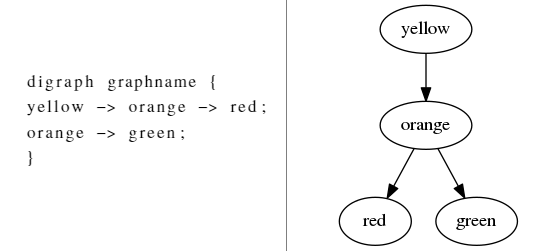
\includegraphics[scale=0.6]{img/Dot.png}
        \caption{DOT kalbos pavyzdys}
        \label{img:dot}
        \end{figure}
        
    \item HTML -- kalba, skirta dokumentų aprašymui, jų turinio pateikimui internete.
    \item CSS -- apibrėžia stilius, naudojamus norint vizualizuoti HTML dokumentą.
    \item LaTeX -- teksto rinkimo sistema, kuri ypač tinka kurti aukštos spausdinimo kokybės moksliniams ir matematiniams dokumentams. Dokumentas yra apibūdinamas LaTeX kalbos elementais ir yra sugeneruojamas PDF failas. LaTeX sistema gali tvarkyti nuorodas į paveikslėlius ar lenteles, gali juos automatiškai išvardyti, todėl tai leidžia vartotojams patogiai valdyti net ir sudėtingų lentelių išdėstymą.\cite{tomassetti2017complete}
\end{itemize}

\subsection{Specializuotųjų kalbų privalumai}

Specializuotosios kalbos yra ribojamos dalykų, kuriuos jos gali padaryti, skaičiumi, tačiau dėl savo specializacijos jos gali pasiekti daug daugiau savo ribotoje srityje. Keli tokių kalbų privalumai yra:
\begin{itemize}
    \item Specializuotosios kalbos yra saugesnės, nes vartotojui pateikiamos tik iš anksto suprogramuotos dalys, naudojant DSL gali iškilti mažiau problemų nei įprastai. Vartotojui nereikia sukti galvos dėl žemo lygio koncepcijų ir sąvokų.
    \item Kai atsiranda klaidų, tai yra tam domenui būdingos klaidos, taigi klaidose kalbama tik apie dalykus, kuriuos gali suprasti domeno ekspertas.
    \item Metakalbų mokytis yra gana paprasta, nes jos yra ribotos apimties, išmokti jas užima mažiau laiko.
    \item Tokias kalbas yra lengviau analizuoti dėl limituotos apimties apibrėžimų. Nors praktiškai neįmanoma garantuoti, kad programa, parašyta C arba Java kalba, laikysis tam tikrų taisyklių (pvz., nepaklius į begalį ciklą), DSL kalboms galima atlikti įvairias analizes.
    \item Specializuotosios kalbos padeda bendrauti su srities ekspertais. Pavyzdžiui kuriant su medicina susijusią projektą, gali tekti bendrauti su gydytojais, kurie tikriausiai yra nesusidūrę su masyvais ar ciklais, tačiau naudojant DSL, kuri aprašo pacientus, temperatūros matus ar kraujospūdį, jie tai galėtų suprasti ir padėti vystyti šį projektą. \cite{tomassetti2017complete}
\end{itemize}


\subsection{Metaprogramavimas}

Programavimas susijęs su metakalbomis vadinamas metaprogramavimu -- tai tokia programavimo technika, kai programos turi galimybę traktuoti kitas kompiuterines programas kaip duomenis. Tai reiškia, kad programa gali būti sukurta generuoti, analizuoti ar transformuoti kitas programas ir netgi modifikuoti save pačią vykdymo metu. Kai kuriais atvejais tai leidžia programuotojams sutrumpinti programos kūrimo laiką, sumažinant kodo eilučių skaičių \cite{czarnecki2000generative}.

Priešdėlis „meta“ šiame kontekste reiškia „aukšto lygio“. Iš apibrėžimo išplaukia du svarbūs dalykai:
\begin{enumerate}
\item Metaprogramavimas susijęs su automatiniu programavimu, dar vadinamu programų generavimu.
\item Metaprogramavimas ir programavimas yra tos pačios srities dalykai, todėl meta programavimas negali būti suprastas neturint programavimo pagrindų.
\end{enumerate}

Metaprogramavimas yra plačiai naudojamas programinės įrangos kūrimo cikle, kur jis atlieka svarbų vaidmenį programų interpretatoriuose ir kompiliatoriuose. Metaprogramavimas kaip konceptualus požiūris nuolat vystosi ir jo principai yra pritaikomi vis aukštesniems abstrakcijos lygiams. Pavyzdžiai apima metamodeliavimą, metadizainą, modeliais pagrįstą inžineriją ir metainžineriją.

Dažnai sakoma, kad metaprograma yra programų generatorius, taigi metaprogramavimas yra automatinis programų kūrimas. Toks teiginys tam tikru mastu motyvuoja metaprogramavimo, kaip specifinės programavimo rūšies poreikį, leidžiantį pasiekti didesnį sistemų kūrimo produktyvumą. Nors yra daug varomųjų jėgų, skatinančių didesnį programinės įrangos projektavimo produktyvumą, dažnai pabrėžiami du dominuojantys veiksniai: (a) projektuojamų sistemų sudėtingumas nuolat auga ir (b) toms sistemoms reikia vis daugiau programinės įrangos turinio.

Metaprogramavimas prisideda prie programų kompleksiškumo valdymo. Kuo daugiau yra naudojami programų generatoriai, tuo mažiau kodo reikia parašyti rankiniu būdu; taigi, kuo sudėtingesnės programinės įrangos sistemos yra sukuriamos, tuo geresnė jų kokybė ir jos gali greičiau pateikti į rinką. Metaprogramavimą galima apibūdinti kaip technologiją, kuri leidžia aiškiai išreikšti numatomą srities kintamumą jau analizės etape ir tokiu būdu įmanoma efektyviai įgyvendinti srities užduotis. Naudojant metaprogramavimo metodus, galima pakeisti požiūrį į projektavimo procesą, bei pamodifikuoti dizainerių atsakomybes bei funkcijas. Pavyzdžiui, metadizaineris gali kurti metaprogramas, kad įgyvendintų pasikartojančias ir sudėtingas užduotis, susijusias su kintamumo valdymu. Tai leistų dizaineriui mažiau pastangų sutelkti programavimui, o daugiau sistemos projektavimo užduotimis.
\cite{štuikys2012meta}

\subsection{Metaprogramavimo įrankiai}
Egzistuoja ne vienas metaprogramavimo ir metakalbų kūrimo įrankis. Keli pavyzdžiai yra:
\begin{itemize}
    \item „Xtext“ -- programavimo kalbų ir DSL kūrimo įrankis, kuriuo galima kurti visaverčius teksto redaktorius tiek bendrosios paskirties, tiek domeno kalboms, be to „Xtext“ redaktoriai yra paruošti JavaScript, VHDL, Xtend ir kitoms kalboms. Patogu tai, kad „Xtext“ IDE yra paremtas populiariu „Eclipse“ IDE, todėl daugeliui programuotojų jis gali atrodyti pažįstamas. „Xtext“ pateikia rinkinį skirtingoms sritims būdingų kalbų ir šiuolaikinių API, skirtą apibūdinti įvairius vartotojų pasirinktos programavimo kalbos aspektus. Vartotojų kalbos kompiliatoriaus komponentai nepriklauso nuo „Eclipse“ ar OSGi ir gali būti naudojami bet kurioje „Java“ aplinkoje. \cite{eysholdt2010xtext}
    \item „JetBrains MPS“ -- domeno kalbų kūrimo įrankis, naudojantis projekcinį redagavimą, leidžiantį vartotojams kurti specializuotųjų kalbų redaktorius su, pvz.: lentelėmis ir diagramomis \cite{JetBrainsMPS}. Apie šį įrankį daugiau bus kalbama vėlesniuose skyreliuose.
    \item „Blockly“ -- „Google“ projektas ir programavimo kalbos JavaScript biblioteka, skirta kurti vizualines programavimo kalbas ir redaktorius blokų pagrindu (angl. \textit{block-based}) \cite{NBCBayArea}. Daugiau apie šį įrankį bus kalbama vėlesniuose skyreliuose.
\end{itemize}

\section{Edukaciniai žaidimai}

Edukaciniai vaizdo žaidimai -- tai vaizdo žaidimai, specialiai sukurti švietimo tikslais arba turintys ugdomąją vertę. Tokie žaidimai yra skirti padėti žmonėms išmokti tam tikrų dalykų, išplėsti sąvokas, sustiprinti vystymąsi, suprasti istorinį įvykį ar kultūrą arba padėti jiems išmokti įgūdžių žaidžiant.

Mokomieji vaizdo žaidimai galėtų vaidinti svarbų vaidmenį mokyklų programose, nes jų pagalba mokiniams gali būti suteikiamos elementariosios žinias ir nauji įgūdžiai. Žaidimų įtraukimas į ugdymo procesą taip pat gali suteikti besimokantiesiems galimybę aktyviai mokytis ir lavinti technologinius įgūdžius, reikalingus jų akademinei ir profesinei karjerai. Keli naujausi tyrimai parodė, kad vaizdo žaidimai, nesvarbu ar juose yra smurto, ar ne, gali padėti vaikams ugdyti intelektinius ir emocinius įgūdžius, kurie palaiko jų akademinius pasiekimus. Šios išvados privertė mokytojus visame pasaulyje pripažinti daugybę žaidimų pranašumų ir į savo programas įtraukti mokomuosius vaizdo žaidimus, kaip ugdymo priemones. \cite{chang2009learning}

Idėja naudoti žaidimus ne linksmybėms, pirmą kartą buvo suformuluota Clark C. Abt knygoje „Rimti žaidimai“ (1975). „Rimti“ žaidimai turi aiškų ir kruopščiai apgalvotą edukacinį tikslą ir nėra skirti vien pramogai. Tokių žaidimų edukacinis tikslas nebūtinai turi būti įtrauktas į žaidimo dizainą, tačiau jį galima priskirti pagal kontekstą, kuriame jis naudojamas. Pavyzdžiui, iš pradžių pramogai sukurtas stalo žaidimas karinio rengimo aplinkybėse gali įgauti tikslą mokyti strateginio mąstymo ir taktinio karo principų. \cite{abt1987serious}

\subsection{Edukacinių žaidimų patrauklumas}

Vaizdo žaidimai labai dažnai būna ilgi, sudėtingi ir sunkiai įveikiami. Nepaisant to, žaidėjai jais džiaugiasi ir ilgą laiką lieka motyvuoti. Mokymasis paprastai taip pat yra ilgas ir sudėtingas procesas, ir, nors žmonės mėgaujasi iššūkiais grįstais žaidimais, jie nemėgsta ir vengia iššūkių keliančios mokymosi patirties mokykliniame ar profesiniame mokyme. Ši priešprieša dar labiau intriguoja, jei manome, kad žaidimo žaidimas visada yra susijęs su mokymusi. Jei skaitmeniniai žaidimai reikalauja mokymosi, pastangų ir noro investuoti laiką ir išteklius ir tai dažnai būna nemalonu kitose situacijose, iškyla klausimas kodėl jie tokie smagūs? Viena svarbiausių vaizdo žaidimų patrauklumo priežasčių yra specifinis jų siūlomas interaktyvumo būdas.

Ši žmogaus ir kompiuterio sąveikos forma gali vykti skirtingais būdais:
\begin{enumerate}
    \item Atskirų įvesčių/išvesčių mikrolygmenyje (pvz.: vartotojas paspaudžia mygtuką ir žaidimo personažas pajuda)
    \item Pasakojimo lygmenyje (pvz.: vartotojas bendrauja su žaidimo elementais, personažais, norėdamas progresuoti žaidime ir sužinoti jo pilną istoriją)
    \item Nustatant ir manipuliuojant žaidimo taisyklėmis (tai apima lygių sudėtingumo  pasirinkimą, sukčiavimą ir naujo žaidimo turinio kūrimą naudojantis redaktoriais)
\end{enumerate}

Visos šias sąveikos turi bendra tai, kad jos suteikia žaidėjui pasitikėjimo savimi jausmą. Žaidėjai suvokia, kaip jų atliekami veiksmai paveikia virtualų žaidimo pasaulį. Šis kontrolės jausmas yra malonus ir skatina tolesnę sąveiką. Trečiasis sąveikos lygis taip pat yra svarbus sklandumo patyrimui esant optimaliai pusiausvyrai tarp iššūkių ir įgūdžių. Kadangi žaidėjai turi skirtingus gabumus ir patirtis, žaidimų gebėjimas prisitaikyti yra nepaprastai svarbus. Kad žaidėjai žaistų žaidimus, jie turi būti „maloniai erzinantys“, t.y. jie turi būti sudėtingi, bet ne pernelyg. Nesėkmės nebūtinai trukdo žaidžiant jausti malonumą, jei pagrįstas praktikos ar unikalaus požiūrio išbandymas leidžia žaidėjui įveikti kliūtis, kurių nepavyko įveikti anksčiau. \cite{breuer2010so}

\subsection{Kūrimo principai}
Nepaisant žaidimų ir mokymosi panašumų, negalima manyti, kad visos žaidimų formos yra vienodai tinkamos mokytis ir kad paprasčiausiai medžiagos pateikimas žaidime padidins mokymosi kiekį ir kokybę. Vien tik įtraukti mokomosios medžiagos į žaidimo koncepciją nepakanka, kad būtų sukurtas įdomus ir efektyvus žaidimas švietimo tikslais. Norint motyvuoti žaidėjus kaip besimokančiuosius, būtina rasti optimalią pramogų ir mokymosi pusiausvyrą.\cite{breuer2010so}

Pasak Chan & Ahern, „kai žmonės yra iš esmės motyvuoti mokytis, jie ne tik mokosi daugiau, bet ir įgyja daugiau teigiamų patirčių“ \cite{chan1999targeting}. Žaidimai atitinka abu šiuos efektyvios mokymosi aplinkos aspektus: jie suteikia naujų potyrių ir gali sužadinti vidinę motyvaciją. \cite{paras2005game}

Ludologijos (žaidimų studijų) tyrinėtojai, žaidimus apibrėžia įvairiai, tačiau dauguma apibrėžimų išryškina tai, jog tai yra žaidėjo pastangos įveikti tam tikrus iššūkius, kad pelnytų apdovanojimą, kuris atvaizduoja sėkmę. Žaidimai turi būti parengti pagal tam tikrus principus, kitaip žaidėjams bus neįdomu ir nenaudinga. Geri žaidimai -- tokie, kurie yra patrauklūs, pakankamai sudėtingi ir nenuspėjami. Barry Fishman apibūdina 10 principų, kurie apibrėžia puikius ugdomuosius žaidimus ir išskirtinę mokymosi aplinką \cite{aguilar2018game}:
\begin{enumerate}
    \item Aiškūs mokymosi tikslai. Gerame žaidime aiškūs tikslai ir instrukcijos padeda žaidėjams progresuoti žaidimo aplinkoje, keliauti per įtraukiančias misijas, lygius ar užduotis. Progreso atvaizdavimas yra vartotojų pritraukimo būdas ir tai suteikia pagrindą tęsti žaidimą toliau. Mokymosi tikslai taip pat turėtų suteikti tam tikrą vertę mokiniams. Tai, kad išmokti dalykai pravers vėliau arba testuose nėra labai patrauklu. Vietoj to, mokytojas/žaidimo kūrėjas turėtų bandyti susieti turinį su atitinkamomis programomis, dabartiniais įvykiais ar tarpdalykiniais kontekstais.
    \item Žaidėjo įtraukimas per veikėjus ir istoriją (angl. \textit{Identity Play}) -- tai daro žaidimą patrauklų ir įdomų. Gerame žaidime žaidėjai valdo įsimintinus personažus ir pasineria į linksmą virtualų pasaulį. Žaidimo užduotys atrodo prasmingos, nes jos yra svarbios istorijai ir veikėjams. Turinys turėtų būti susietas su kokiu nors kontekstu; priešingu atveju mokiniai gali nesuprasti mokomų įgūdžių ir žinių prasmės. Taigi, pavyzdžiui, vietoj vien mokymosi kaip programuoti, mokiniai turėtų išmokti mąstyti ir elgtis kaip programuotojai.
    \item Vertinimo įtraukimas į žaidimo eigą. Žaidėjo įgūdžiai ir pasirinkimai kiekvieną akimirką yra stebimi, todėl žaidimai paprastai prisitaiko prie naujai įgytų žinių ir sugebėjimų, koreguojant lygių ar dalių sunkumą. Gerai suplanuota mokymosi aplinka integruoja dažnus, bet minimalius žinių vertinimus. Užuot vertinus didelį kiekį žinių vienu kartu, vertėtų įkomponuoti smulkias, mažiau įkyrias užduotis į natūralų kurso/žaidimo srautą. Taip mokiniai/vartotojai gali jaustis labiau atsipalaidavę ir sudominti.
    \item Vidinė ir išorinė motyvacija. Žaidimai tenkina vartotojus ir juos žavi, nes jie kelia iššūkius -- žmonėms patinka spręsti problemas ir įveikti kliūtis. Tyrėjai teigia, kad įsitraukimą į žaidimą palaiko vidinė motyvacija, tačiau kokybiški žaidimai juos dar labiau įtraukia suteikiant jiems atitinkamą atlygį (išorinė motyvacija). Žaidimo metu atlygis turėtų būti minimalus, tik toks, kad žaidėjai išliktų motyvuoti. Jei atlygis yra per daug reikšmingas, žaidėjai gali prarasti susidomėjimą. \cite{pavluswe}
    \item Autonomijos palaikymas. Sėkmingi žaidimai pateikia žaidėjui intriguojančius ir sudėtingus pasirinkimus. Pavyzdžiui, žaidėjai gali pasirinkti savo personažą ar kelią, kuriuo jie eis, norėdami užbaigti užduotį. Žaidybinėje mokymosi aplinkoje mokiniai dažnai pasirenka savo kursų turinio, studijų dalykų ar net užduočių ir vertinimų kelią.
    \item Bendrystės skatinimas. Kelių žaidėjų (angl. \textit{Multiplayer}) žaidimai yra nepaprastai populiarūs. Tokio tipo žaidimuose žaidėjai dirba kartu, siekdami bendro tikslo, remdami savo komandą, prisidėdami savo įgūdžiais. Šio tipo sąveika skatina bendrystės jausmą, kuris motyvuoja tęsti žaidimą ir įgūdžių tobulinimą. Vadovaujantis Vygotsky sociokultūrine teorija, mokymasis glaudžiai susijęs su socialiniais ir kultūriniais kontekstais. \cite{wertsch1992ls}
    \item Kompetencijos palaikymas. Sėkmingi žaidimai palaipsniui didina sudėtingumą ir palaiko žaidėjus jiems įgyjant naudingų įgūdžių. Gerai suplanuotuose kursuose mokiniai užsiima turiniu, kuris yra sudėtingas, bet taip pat ir įgyvendinamas kartu su mokytojų ir bendraamžių pagalba. \cite{vygotsky1980mind}
    \item Produktyvios nesėkmės. Žaidimai neturėtų per daug bausti vartotojo, jei šiam nepasiseka. Jei veikėjas miršta arba jam kitaip nepasiseka, žaidėjui paprastai leidžiama paleisti žaidimą iš naujo arba nuo tam tikros vietos ir bandyti dar kartą. Gerame žaidime vartotojai mokosi iš savo klaidų ir dažniausiai jiems pasiseka, kai jiems suteikiama dar viena galimybė atlikti užduotį. Neturint „atstatymo mygtuko“, nesėkmė tradicinėje mokyklos aplinkoje gali sumažinti mokinio motyvaciją. Negana to, švietimo sistema linkusi netiesiogiai skatinti sukčiavimą, nes nėra leidžiama padaryti klaidų. Kokybiška mokymosi aplinka suteikia mokiniams/studentams galimybę dažnai pasitikrinti savo žinias ir mokytis iš klaidų prieš susiduriant su svaresniais vertinimais ir užduotimis. Tokioje aplinkoje nesėkmė laikoma mokymosi proceso dalimi, o ne jo pabaiga.
    \item Skatinimas tyrinėti. Geri žaidimai paprastai yra kupini paslapčių, ir kai kurie žaidėjai jas tyrinėja daugybę valandų, kad jas visas išsiaiškintų. Taip lavinamas mąstymas, problemų sprendimo radimo sugebėjimai ir žaidėjas išlieka sudomintas, bei motyvuotas.
    \item Praktika. Dažnai užduodamos užduotys ir jų atkartojimas žaidime padeda labiau įsisavinti informaciją ir ne taip greitai ją pamiršti. Kuo daugiau užduočių yra sprendžiama, kuo daugiau praktikos įgaunama, tuo geriau galima išmanyti tam tikrą sritį. \cite{kenney_2020}
\end{enumerate}

Norint palaikyti tinkamą informacijos tėkmę, mokymosi aplinka turi tiksliai atitikti kiekvieno mokinio įgūdžių lygį, užduotys turi būti pateikiamos su aiškiais tikslais ir dažnu grįžtamuoju ryšiu. Apskritai, mokymosi aplinkai išskiriami tokie reikalavimai:
\begin{itemize}
    \item Reiktų suteikti didelį kiekį veiklų ir palaikyti dažną grįžtamąjį ryšį.
    \item Reiktų turėti konkrečius tikslus ir iš anksto nustatytas procedūras.
    \item Svarbu motyvuoti.
    \item Vertėtų suteikti nuolatinį iššūkio jausmą, kuris nėra nei toks sunkus, kad sukurtų beviltiškumo ir nusivylimo jausmą, nei toks lengvas, kad sukeltų nuobodulį.
    \item Reiktų suteikti tiesioginio įsitraukimo jausmą dirbant ties užduotimi.
    \item Turi būti pateikiami reikalingi įrankiai, kurie tinka vartotojui ir užduočiai taip, kad padėtų ir neblaškytų dėmesio.
    \item Svarbu išvengti pašalinių įsikišimų, kurie trukdytų žmogui įgauti subjektyvią patirtį.
\end{itemize}

Priimant šiuos reikalavimus mokymosi aplinkai, tektų pripažinti, kad mokymasis yra neatsiejamas nuo žaidimų. Žaidimai gali atrodyti tokie smagūs, kad jie užmaskuoja tai, kiek iš tikrųjų reikia išmokti, norint sėkmingai šiuos žaidimus žaisti. \cite{houser1998learning}

\subsection{Mokytojai}
Mokomieji žaidimai skiriasi nuo įprastinių, tuo, kad edukacinių žaidimų dalyvių yra daugiau nei paprastuose: į dalyvių sąrašą įtraukiami ir mokytojai.

Tam, kad mokytojams būtų patogu prisidėti prie edukacinių žaidimų kūrimo, atsiranda keletas reikalavimų sistemai:
\begin{itemize}
    \item Sistemą arba IDE, turėtų būti paprasta naudoti ir paleisti. Ne visi mokytojai turi geras kompiuterinio raštingumo žinias, todėl ne kiekvienas supranta sudėtingas sistemas, turinčias daug funkcijų. Mokytojams taip pat reikia paaiškinti mokiniams kaip naudotis sistema, todėl kuo ji yra aiškesnė, tuo mažiau laiko yra sugaištama šiems mokymams.
    \item Mokytojui turi būti suteikta galimybė stebėti mokinio pažangą ir įvertinti jo įgytas žinias. Informacija apie tai, kaip gerai mokinys vykdo užduotis ir įsisavina informaciją turi būti prieinama ir pateikta mokytojui. Vertinimo sistema taip pat gali būti įdiegta pačiame žaidime -- gali būti rodomas surinktų taškų skaičius, pereitų lygių skaičius, prarastos gyvybės ar kt.
\end{itemize}

\section{„JetBrains MPS“}

„JetBrains MPS“ -- „JetBrains“ kompanijos kurtas įrankis skirtas DSL kalboms kurti. Jis naudoja projekcinį redagavimą, kuris leidžia vartotojams peržengti kalbos analizatorių (angl. \textit{parser}) ribas ir kurti domeno kalbų redaktorius. 
Programuojant MPS įrankiu kuriama specializuotoji kalba paprastai yra mažiau sudėtinga nei bendrosios paskirties kalba, tokia kaip Java ar C. Paprastai specializuotosios kalbos kuriamos glaudžiai bendradarbiaujant su tos srities specialistais, kuriems ta kalba yra kuriama. Daugeliu atvejų tokios kalbos yra skirtos naudoti ne programuotojams, o būtent tos srities atstovams. \cite{JetBrainsMPS}.

Edukacinių žaidimų kontekste, MPS yra labiau skirtas vyresniems mokiniams ar studentams ir dėstytojams, nes jie gali mokėti naudotis sudėtingesniu IDE ir gali labiau norėti naudoti tekstinę kalbą, o ne vaizdinius kodų blokus.

\subsection{Specializuotųjų kalbų ir įprasto kodo darna}
Yra du skirtingi būdai, kaip integruoti tradicinį kodą ir specializuotosios kalbos kodą MPS:
\begin{enumerate}
\item Pirmasis būdas yra saugoti DSL kodą ir įprastą kodą atskiruose failuose. Tuomet automatinis kodo generatorius DSL kodą išverčia į programavimo kalbos kodą, arba programa gali įkelti konkrečiai sričiai skirtą kodą ir jį vykdyti. Šis būdas su atskirta bendrosios paskirties kalba bei atskiru DSL kodu vadinamas išorine specializuotąja kalba (angl. \textit{external DSL}). Vienas išorinės DSL pavyzdžių yra SQL.
\item Antrasis metodas yra DSL kodą ir bendrosios paskirties kodą maišyti tame pačiame faile, tuomet jų integracija yra griežtesnė. DSL pakartotinai naudoja bendrosios paskirties kalbos gramatiką, analizatorių bei esamas pagrindinės kalbos išplėtimo parinktis. Tokiam turiniui apibūdinti naudojamas terminas vidinė specializuotoji kalba (angl. \textit{internal DSL}).\cite{JetBrainsMPS}
\end{enumerate}

\subsection{Specializuotųjų kalbų projektavimas}
MPS, kaip ir daugelis kitų kalbų kūrimo įrankių, siūlo DSL rinkinį įvairiems kalbų aspektams apibrėžti. Tai apima struktūrą, redaktorių, tipų sistemą, generatorių, taip pat ir IDE funkcionalumų palaikymą. \cite{10.1145/2500828.2500846}

\subsubsection{Abstrakti sintaksė}
Pirmasis žingsnis apibrėžiant naują specializuotąją kalbą MPS programoje yra nurodyti struktūrą (dar vadinama abstrakčia sintakse). Tai primena objektinį programavimą, kalbos sąvokos yra panašios į klases. Sąvokos MPS atstovauja abstraktaus sintaksės medžio (angl. \textit{Abstract syntax tree (AST)})(toliau vadinamas AST) mazgų tipus ir apibrėžia savybes, vaikus, metodus ir ryšius, kuriuos mazgai gali turėti. MPS naudoja kelis kalbos aspektus abstrakčiai sintaksei apibrėžti: \textit{struktūros} aspektas nusako sąvokas, jų savybes ir ryšius, \textit{apribojimai} riboja leistiną aibę savybių ir nuorodų verčių, o \textit{elgesys} (angl. \textit{behavior}) metodus sieja su sąvokomis \cite{10.1145/2500828.2500846}.

Taigi, naudojant naująją DSL programai kurti, reikia suformuoti tos kalbos sąvokas, priskirti reikšmes sąvokų savybėms ir susieti programos mazgus pagal ryšius, apibrėžtus šių savokų. Visa tai palaiko galingi redaktoriai, kuriuos galima savarankiškai apibrėžti savo kalbai.

Ne visi DSL kūrimo įrankiai abstraktų sintaksės medį vaizduoja taip pat kaip MPS. „Scratch“ ir „Blockly“ sistemos, vaizdinių redaktorių pagalba skiria medžio mazgams savitą formą. Šakninių mazgų blokus galima dėti tik ant kitų viršaus. Tai suteikia galimybę intuityviai konstruoti AST.

\subsubsection{Konkreti sintaksė}
Antrasis etapas -- savokų redaktoriaus apibrėžimas. Kadangi MPS aplinkoje kodas niekada nėra vaizduojamas kaip paprastas tekstas, MPS kalbos niekada nėra formatuojamos ar analizuojamos (angl. \textit{parsed}), taigi joms nereikia nustatyti gramatikos. Tai įgalina naudojimąsi lentelėmis ar matematiniais simboliais. Vietoj analizatoriaus yra apibrėžiamas redaktorius kuriamų kalbų sąvokoms -- vaizdinė AST mazgų reprezentacija. MPS redaktorius leidžia programuotojui apibrėžti savo naujosios kalbos konstrukcijos redaktorių, arba pamodifikuoti esamų kalbų sąvokų redaktorius. Redaktoriai gali būti skirstomi į skirtingus modulius, kad būtų galima pakartotinai naudoti vaizdinės sintaksės elementus, taip pat keli redaktoriai gali apibrėžti specifinę sąvoką, o tai leidžia kalbos kūrėjui pasirinkti tinkamiausią žymėjimą domenui, kuriame dirbama \cite{10.1145/2500828.2500846}.

Redaktorius padeda išdėstyti kiekvienos sąvokos poziciją jame. Galima apibrėžti, kurios dalys yra pastovios/konstantos, pavyzdžiui, skliausteliai ar kitos detalės, o kurios dalys yra kintamos ir jas reikia įrašyti vartotojams.

\subsubsection{Kodo transformacija}
MPS kalbos nusako taisykles, kaip transformuoti turimą informaciją į žemesnio lygio kalbas arba paprastą tekstą. Kodo generavimo procesą sudaro dvi fazės:
\begin{enumerate}
\item Pirmoje fazėje naudojamas šablono pagrindu pagrįstas „modelis modeliui“ (angl. \textit{model-to-model}) transformacijos variklis, kuris leidžia redukuoti programos kodą į tikslinę kalbą, remiantis generatoriaus apibrėžtomis taisyklėmis. Tikslinė kalba gali būti dar labiau redukuota remiantis jos pačios redukcijos taisyklėmis ir taip toliau.
\item Kai redukcija nebegali būti taikoma tolesniam modeliui, pradedama antroji fazė, kuri naudoja teksto generatorių, kuris konvertuoja galutinį modelį į įprastą programos tekstą. Šį tekstą jau galima pateikti kompiliatoriui. \cite{10.1145/2500828.2500846}
\end{enumerate}


Kalbos generatorių sudaro du pagrindiniai elementai: \textit{konfigūracijų žemėlapis} (angl. \textit{mapping configurations}) apibrėžia, kokiais šablonais ir kokiame kontekste yra apdorojamos sąvokos, o \textit{šablonai} apibrėžia kodą tiksline kalba, kuri pakeis nurodytą šaltinio sąvokos dalį.

\subsection{Bazinė kalba}
MPS glaudžiai susijęs su programavimo kalba Java. Pats MPS yra sukurtas Java pagrindu, ir veikia Java dialekto, vadinamo bazine kalba (angl. \textit{Base Language}), pagalba. Ši kalba palaiko tokias kalbos ypatybes kaip aritmetika, ciklai, funkcijos, sąlygos sakiniai, kintamieji ir kt.

Bazinė kalba taip pavadinta, nes ji yra neblogas pagrindas daugeliui kitų kalbų, kurioms reikalingos išvardintos kalbos ypatybės. Ji gali būti naudojama keliais būdais: galima išplėsti šią kalbą, kad ja remiantis būtų sukurta kita, nauja kalba, galima naudoti jos sąvokas savo programose, arba taip pat ir sugeneruoti savo parašytą kodą į bazinę kalbą.

\subsection{Privalumai}

Pirmasis MPS privalumas yra tas, kad projekcinės kalbos turi redaktorius su apibrėžta griežta sintakse, kuri gali padėti pradedantiesiems programuotojams. Išmani kodo užbaigimo (angl. \textit{code completion}) funkcija  gali būti labai patogi, nes didesnės kodo dalys gali būti įterptos automatiškai, todėl sintaksė gali pasirodyti aiškesnė, nereikia per daug rašyti ranka. Vartotojams nereikia rūpintis specialių simbolių, tokių kaip skliaustelių ar kabliataškių, įterpimu. Redaktorius taip pat turi iš anksto nustatytą išdėstymą, kuris pats pasirūpina tarpais ir įtraukomis.

Sintaksės paryškinimai (angl. \textit{syntax highlighting}) taip pat gali atvaizduoti santykius tarp mazgų, ne tik jų sintaksę. Redaktoriuje pridedamas papildomas tekstas gali keistis, vartotojui keičiant kodą, pvz. kai trūksta kažkokio mazgo, toje vietoje gali būti pridėta tiksli užuomina, kuri padės vartotojui tai ištaisyti, o kai kodas teisingas, užuomina dingsta. Projekcinio kodo nereikia analizuoti (angl. \textit{parse}), todėl skirtingas kalbas galima derinti laisviau. Taip pat  redaktoriuje yra palaikomi vaizdiniai elementai, tokie kaip lentelės ar diagramos.

Dėl tipų sistemos ir duomenų srauto (angl. \textit{typesystem and dataflow}) aspektų lengviau atlikti kai kuriuos patikrinimus, todėl kai kurios klaidos gali būti nedelsiant pranešamos joms įvykus ir yra sunkiau parašyti neteisingą kodą. \cite{klimevs2016domain}

\subsection{Trūkumai}

Dauguma problemų kyla dėl to, kad MPS kalbos kodas nėra paprastas tekstas, o atskiri MPS modeliai, kuriuose gali būti daugiau šakninių mazgų, saugomų viename XML dokumente. Projekcinį kalbos kodą galima skaityti ir rašyti tik „IntelliJ IDEA“ su „MPS“ įskiepiu (angl. \textit{plugin}) arba „JetBrains MPS“ programose. Kalba taip pat turi būti supakuota ir importuota į IDE. Kodas iš MPS redaktoriaus gali būti nukopijuotas kaip tekstas, tačiau kai reikia įterpti kodą kaip paprastą tekstą atgal į MPS redaktorių, reikia įdėti papildomų pastangų. 

Programuotojams, įprastai naudojantiems teksto redaktorius, reikia laiko priprasti prie numatytojo MPS redaktoriaus. Kodo konstravimas naudojantis iš anksto apibrėžtomis kalbos sąvokomis tikrai jaučiasi kitaip, nei kodo rašymas paprastame teksto redaktoriuje. Vartotojams, naudojantiems sistemą, taip pat nėra lengva priprast prie tokio redaktoriaus. „Scratch“ arba „Blockly“ kalbų kūrimo redaktoriai yra akiai malonesni ir patogesni. Jie abu yra skirti mokymams, todėl jų grafinė vartotojo sąsaja yra pritaikyta mokiniams (\ref{img:editors} paveikslėlis).

\begin{figure}[H]
    \centering
    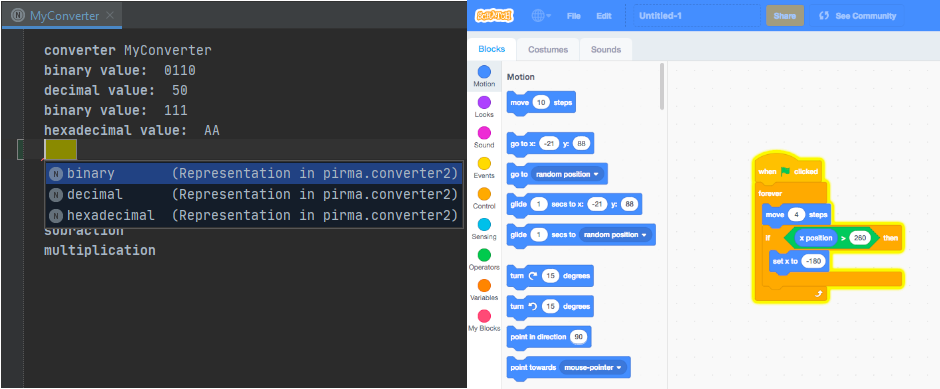
\includegraphics[scale=0.6]{img/editors.png}
    \caption{Kairėje: MPS redaktorius, dešinėje: „Scratch“ redaktorius }
    \label{img:editors}
\end{figure}

Be to, neįmanoma valdyti versijų be MPS VCS įskiepio, kuris supranta AST XML vaizdavimą. Programuotojas negali jungti pakeitimų rankiniu būdu ir net nedideli pakeitimai, neturintys įtakos kodo išvaizdai redaktoriuje, gali nutraukti kai kurias AST nuorodas ir padaryti kodą neveikiančiu. Taigi pakeitus versiją gali būti sugadintas esamas kodas. Kad kalbos evoliucija būtų įmanoma, MPS pateikia migracijos funkciją kodui transformuoti į skirtingas kalbos versijas.

Ateities versijose MPS kūrėjai planuoja sukurti galimybę MPS naudoti WEB programose, tačiau nėra aišku, ar MPS tikrai vystysis šia kryptimi, be to tai gali užtrukti ne vienerius metus. Tai neleidžia pateikti kalbos internete su pritaikyta ir supaprastinta vartotojo sąsaja.\cite{klimevs2016domain} 

\section{„Blockly“}

\subsection{Vizualinės programavimo kalbos}

Vizuali programavimo kalba (VPL) yra programavimo kalba, leidžianti vartotojui kurti programas jas grafiškai manipuliuojant.
% \cite{jost2014graphical}.
Keletas bendrų VPL sąveikos bruožų yra:
\begin{itemize}
    \item Blokų vilkimas ekrane,
    \item Srautų, būsenos diagramų ir kitokių komponentų jungimo naudojimas,
    \item Piktogramų naudojimas ir netekstinis atvaizdavimas
\end{itemize}

Daugelis VPL vis tiek naudoja tekstinius laukus arba juos sujungia su vaizdais. Kiekviena vizuali programavimo kalba turi savo gramatiką ir žodyną. Kartu jie apibrėžia sąvokų rinkinį, kurį galima lengvai išreikšti ta kalba. Gramatika yra vaizdinė metafora, kurią naudoja kalba: blokai, jungimo būdai ir kt. Žodynas yra piktogramų, blokų ar kitų komponentų rinkinys, leidžiantis išreikšti idėjas. \cite{pasternak2017tips}

\subsection{„Blockly“ biblioteka}

„Blockly“ yra programavimo kalbos JavaScript biblioteka, kuri prideda vaizdinį kodo redaktorių WEB ir mobiliųjų programoms. Šis redaktorius naudoja besijungiančius grafinius blokus kodo sąveikoms, tokioms kaip kintamieji, loginės išraiškos, kilpos ir kt., atvaizduoti. \cite{introduction to blockly} Paprastai jis veikia žiniatinklio naršyklėje ir vizualiai primena „Scratch“ kalbą. Jis taip pat diegiamas mobiliesiems „Android“ ir „iOS“ operacinėms sistemoms, nors tose platformose nėra galima naudotis visomis naršyklės funkcijomis.

„Blockly“ naudoja blokus, kurie gali sugeneruoti JavaScript, Lua, Dart, Python ar PHP kodą. Jis taip pat gali būti pritaikytas generuoti kodą bet kuria kita tekstine programavimo kalba \cite{NBCBayArea}. „Blockly“ nėra nei pilna kalba, nei programa, paruošta galutiniams vartotojams. Šioje bibliotekoje pateikiama programavimo gramatika ir reprezentacijos, kurias kūrėjai gali naudoti savo programose. Kodas vaizduojamas blokais, kuriuos galima vilkti ekrane. Šie blokai turi jungties taškus, todėl juos galima pritvirtinti prie kitų blokų ir sujungti grandinėmis. „Blockly“ nepateikia pilno blokų žodyno ar vykdymo aplinkos -- kūrėjai turi patys kurti savo žodyną ir nuspręsti, kaip veiks sugeneruotas kodas  \cite{pasternak2017tips}.

Bendrai, norint sukurti „Blockly“ programą reikia atlikti tokius veiksmus:
\begin{itemize}
    \item Integruoti „Blockly“ redaktorių. Paprasčiausias „Blockly“ redaktorius susideda iš įrankių rinkinio blokų tipams saugoti ir darbo srities, skirtos blokams tvarkyti.
    \item Sukurti savo programos blokus. Į savo programą įtraukus „Blockly“, reikia sukurti reikiamus blokus atitinkamai sričiai, tada pridėti juos prie „Blockly“ įrankių rinkinio.
    \item Sukurti likusią programos dalį. Pats „Blockly“ yra tik būdas generuoti kodą. Vartotojas pats nusprendžia, ką daryti su tuo kodu.
\end{itemize}

\subsubsection{Dažniausiai naudojami žodynų stiliai}
\label{section:dazniausiStiliai}

Blokų kalboms dažniausiai naudojami stiliai: paveikslėlių, natūralios kalbos ir kompiuterių kalbos:
\begin{itemize}
    \item Paveikslėlių blokai remiasi vaizdais, o ne tekstu, kad perteiktų tai, ką blokai daro. Jie taip pat gali įtraukti skaičius ir nedidelį teksto kiekį. Šie blokai gali būti veiksmingi norint pasiekti jaunesnius vartotojus: vaikai, neišmokę skaityti, vis tiek gali juos naudoti rašydami kodą.
    
    Nors paveikslėlius vartotojams gali būti lengviau suprasti nei tekstą, tai taip pat sukuria daugiau apribojimų blokams ir tam, ką jais galima išreikšti. Gali būti sunku perteikti abstrakčias sąvokas paveikslėliais, sąlygas sunku apibrėžti be teksto. Net aiškius paveikslėlius vartotojui gali būti sunku prisiminti, jei jų yra per daug, todėl daugeliui panaudojimo atvejų tinka nedidelis paprastų blokų rinkinys \cite{pasternak2017tips}. Paveikslėlių blokų pavyzdį galima matyti „Codelab“ programoje (\ref{img:codeLab} paveikslėlis).
    
    \begin{figure}[H]
    \centering
    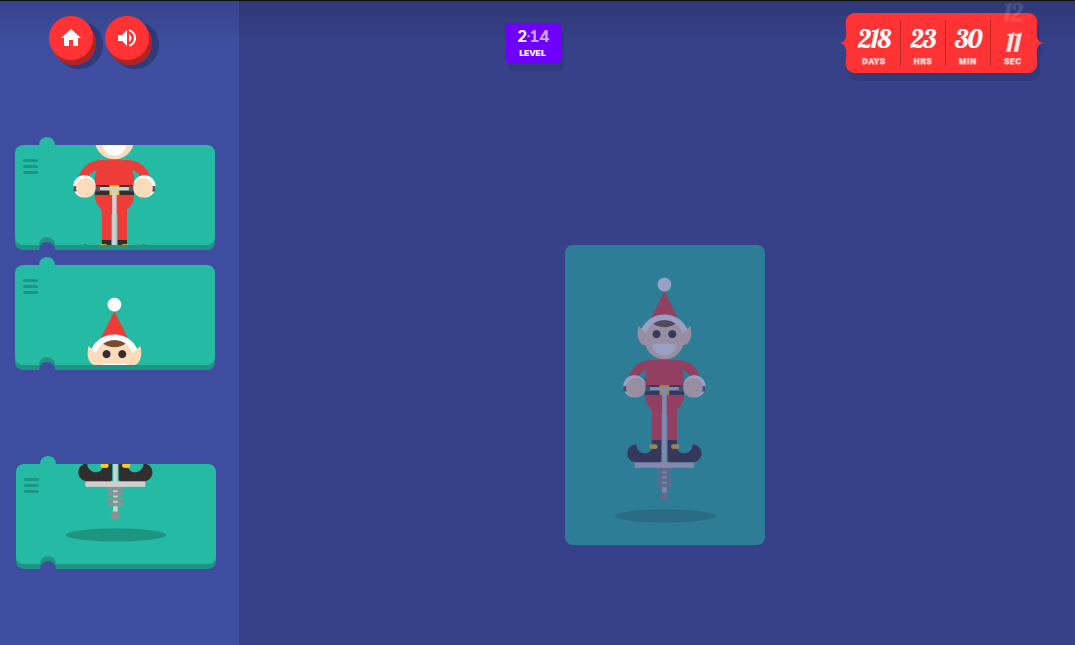
\includegraphics[scale=0.3]{img/santatracker.png}
    \caption{„Codelab“ programa, naudojanti paveikslėlių blokelius \cite{codeLab}}
    \label{img:codeLab}
    \end{figure}
    
    \item Natūralios kalbos blokuose naudojami įprasta kalba užrašyti sakiniai. Blokai, kuriuose naudojami tokie sakiniai gali būti naudojami sudėtingesnėms sąvokoms išreikšti, tačiau vartotojai vis tiek jaučiasi jaukiai ir gali naudotis programa intuityviai. Daugeliui vartotojų sakiniai yra lengviau skaitomi ir suprantamesni už programinį kodą, todėl gerai suprojektuotuose projektuose bet kokio amžiaus vartotojai gali patirti įdomius iššūkius. „Scratch“ \cite{scratch}, populiari blokinė vizualinio programavimo kalba, skirta vaikams ir paaugliams, yra puikus šios kategorijos pavyzdys, išlaikęs ilgalaikį patrauklumą (\ref{img:scratch1} paveikslėlis) \cite{pasternak2017tips}.
    
    \begin{figure}[H]
    \centering
    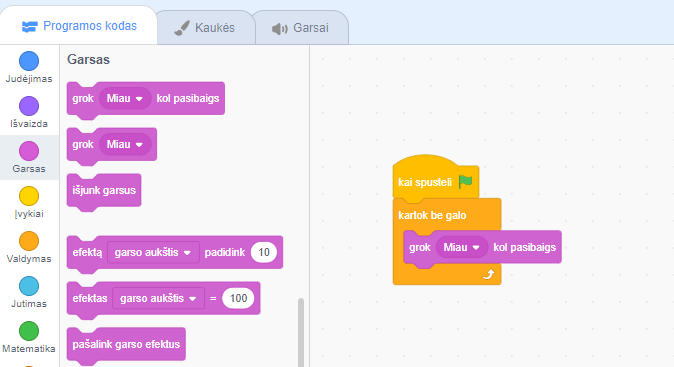
\includegraphics[scale=0.6]{img/scratchPvz.png}
    \caption{„Scratch“ blokai, reiškiantys jog spustelėjus vėliavėlę, „miau“ garsas bus grojamas be galo}
    \label{img:scratch1}
    \end{figure}
    
    \item Dar vienas būdas kurti kalbas yra naudoti blokus, kurie atrodo kaip esama tekstinė programavimo kalba (\ref{img:computerLanguage} paveikslėlis). Blokinių variantų egzistavimas gali padėti mokiniams priprasti prie tam tikros programavimo kalbos ir taip lengviau pereiti prie tekstinio programavimo \cite{pasternak2017tips}.
    
    \begin{figure}[H]
    \centering
    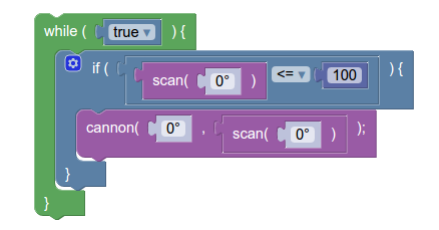
\includegraphics[scale=0.6]{img/computerLanguagePvz.png}
    \caption{„Blockly“ JavaScript kalbos blokai}
    \label{img:computerLanguage}
    \end{figure}

\end{itemize}

\subsubsection{Vartotojo sąsaja}

Numatytąją „Blockly“ redaktoriaus grafinę vartotojo sąsają (angl. \textit{GUI}) sudaro „įrankių dėžė“, kurioje yra skirtingų rūšių blokai, ir darbo sritis, į kurią vartotojas gali vilkti blokus ir juos pertvarkyti (\ref{img:toolbox} paveikslėlis). Darbo srityje pagal numatytus nustatymus taip pat gali būti ir šiukšliadėžė blokams ištrinti. Redaktorių galima lengvai modifikuoti, kad būtų galima pritaikyti ir apriboti galimas redagavimo funkcijas ir blokus pagal tam tikrą specializuotąją sritį.

\begin{figure}[H]
    \centering
    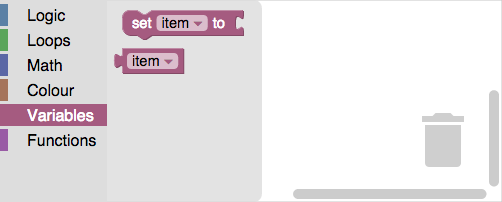
\includegraphics[scale=0.6]{img/toolbox.png}
    \caption{„Blockly“ vartotojo sąsaja}
    \label{img:toolbox}
\end{figure}

„Blockly“ apima vaizdinių blokų rinkinį, skirtą įprastoms operacijoms, bet jį galima pritaikyti ir kitai specializuotajai sričiai pridedant daugiau blokų. Naujiems blokams reikalingas bloko apibrėžimas ir generatorius. Apibrėžimas apibūdina bloko išvaizdą (vartotojo sąsają), o generatorius -- bloko vertimą į vykdomąjį kodą. Apibrėžimai ir generatoriai gali būti parašyti „JavaScript“ arba naudojant vaizdinį blokų rinkinį „Block Factory“, leidžiantį naujus blokus apibūdinti naudojant esamus vaizdinius blokus; taip siekiama palengvinti naujų blokų kūrimą.

\subsubsection{Integracija}
Įtraukti „Blockly“ į savo projektą galima per „npm“ paketų tvarkyklę (angl. \textit{„package manager“}) arba įterpus šią eiluę HTML faile: 
\begin{lstlisting}[language=HTML]
<script src="https://unpkg.com/blockly/blockly.min.js"></script>
\end{lstlisting}
Naudojantis antruoju būdu, „Unpkg“ gauna naujausią paskelbto kodo versiją, todėl naudojant šį metodą nėra galimybės kontroliuoti, kokia versija bus pasirinkta.

Taip pat galima atsisiųsti visą šaltinio kodą iš „GitHub“. Tačiau, norint gauti naujausius „Blockly“ naujinimus ir pataisymus, reiktų reguliariai sinchronizuoti šią saugyklą.

\subsubsection{Naujų blokų kūrimas}

„Blockly“ turi daug iš anksto paruoštų blokų: nuo matematinių funkcijų iki ciklinių struktūrų, tačiau norint sąveikauti su kitomis išorinėmis programomis, reikia sukurti sričiai pritaikytus (angl. \textit{„custom“}) blokus, kad būtų suformuotas API. Pavyzdžiui, kuriant piešimo programą gali tekti sukurti „R spindulio apskritimo piešimo“ bloką. Daugeliu atvejų paprasčiausias būdas yra tiesiog surasti panašų, jau egzistuojantį bloką, į reikiamą, jį nukopijuoti ir modifikuoti pagal poreikį.

\subsubsubsection{Blokų apibrėžimas}

Pirmasis žingsnis kuriant bloką yra nurodyti jo formą, laukus ir jungimosi taškus. Lengviausias būdas tai padaryti yra pasinaudoti „Blockly Developer Tools“, bet taip pat galima parašyti šį kodą ranka, išanalizavus API.

„Blockly Developer Tools“ yra programuotojų įrankis, kuris automatizuoja „Blockly“ konfigūravimo proceso dalis, įskaitant naujų blokų kūrimą, įrankių dėžės sukūrimą ir „Blockly“ darbo srities konfigūravimą. Šiame įrankyje yra „Block Factory“ skirtukas, kuriame ir galima kurti naujus blokus. Pagal tai kaip yra sukonfigūruotas blokas vizualiame redaktoriuje, yra sugeneruojamas kūrimo bloko kodas, kurį galima įterpti į savo programinį kodą arba išsaugoti visą naujų blokų biblioteką ir ją integruoti į savo projektą (\ref{img:developerTools} paveikslėlis). \cite{blockly-developer-tools}

\begin{figure}[H]
    \centering
    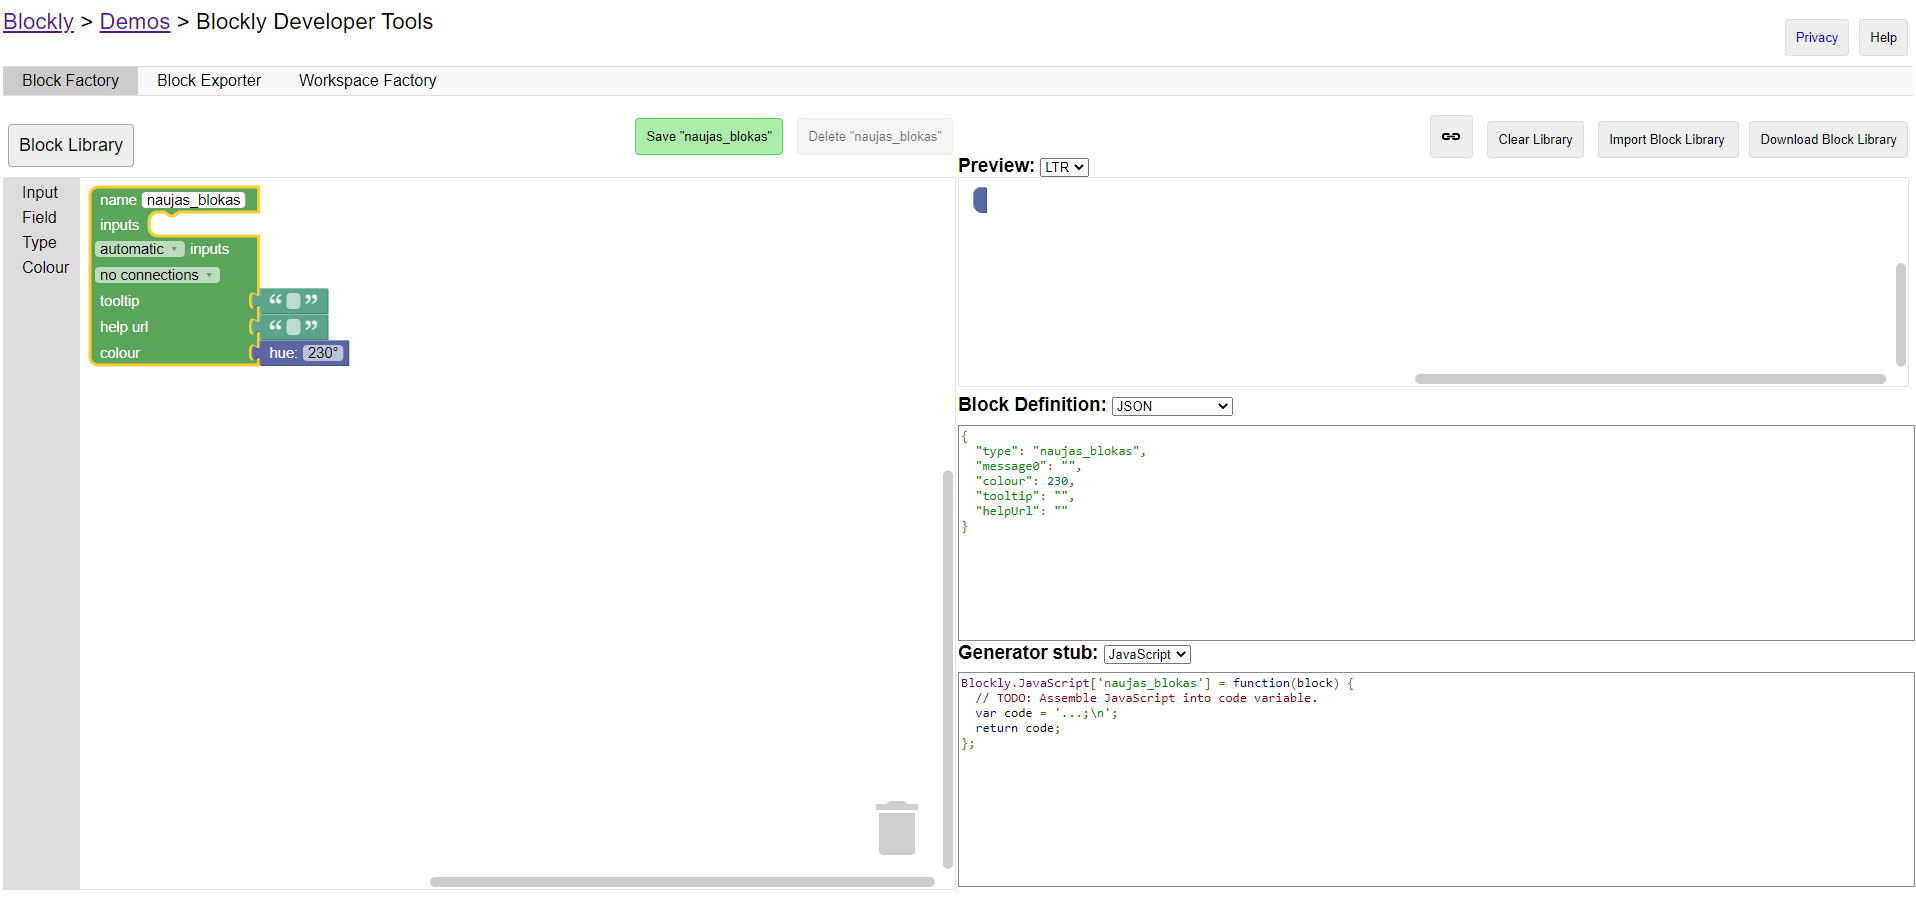
\includegraphics[scale=0.3]{img/developerTools.png}
    \caption{„Blockly Developer Tools“ blokų generavimo skirtukas}
    \label{img:developerTools}
\end{figure}

Pasirinkus nesinaudoti „Blockly Developer Tools“, aprašyti blokus įmanoma dviem būdais: JSON objektais arba JavaScript funkcijomis. JSON formatas sukurtas siekiant supaprastinti lokalizavimo procesą kuriant kalboms, kur naudojamos skirtingos žodžių tvarkos. Deja JSON formatu negalima tiesiogiai apibrėžti sudėtingesnių funkcijų, tokių kaip mutatoriai ar validatoriai. Jos turi būti parašytos platformos gimtuoju kodu, JavaScript, Java arba Swift, paprastai kaip plėtiniai.

WEB puslapyje JSON formatas įkeliamas naudojant „initJson“ funkciją. Tai taip pat leidžia maišyti anksčiau minėtus formatus. Pageidautina, jei įmanoma, bloką apibrėžti naudojant JSON, o „JavaScript“ naudoti tik toms blokų apibrėžimų dalims, kurių JSON nepalaiko. Žemiau pateikiamas bloko, kuris daugiausia apibrėžtas naudojant JSON, tačiau išplėstas naudojant JavaScript API, pavyzdys (\ref{img:blockJson} paveikslėlis).

\begin{figure}[H]
    \centering
    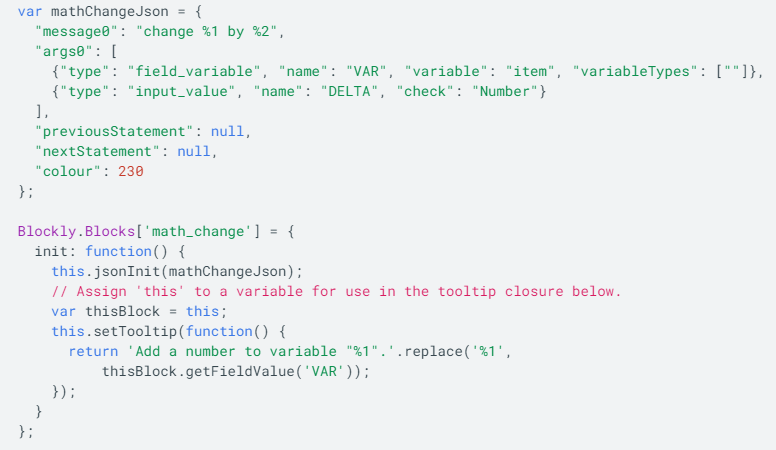
\includegraphics[scale=0.6]{img/blockJsonJS.png}
    \caption{Blokas, apibrėžtas JSON ir JavaScript kalbomis}
    \label{img:blockJson}
\end{figure}

Vartotojai gali sukurti blokų sekas naudodami „nextStatement“ ir „previousStatement“ jungtis. Standartiniame „Blockly“ išdėstyme šios jungtys yra viršuje ir apačioje, blokai išdėstyti vertikaliai. \cite{define-blocks}

\subsubsubsection{Kodo generavimas}
Antrasis žingsnis blokų kūrimo procese yra sukurti generatoriaus kodą, kad nauji blokai būtų išversti į programavimo kalbą (JavaScript, Python, PHP, Lua ar Dart). Generatorius aprašomas ne pernelyg sudėtingai, tipiškas bloko kodo generatorius atrodo kaip \ref{img:generatingCode} paveikslėlyje. \cite{generating-code}

\begin{figure}[H]
    \centering
    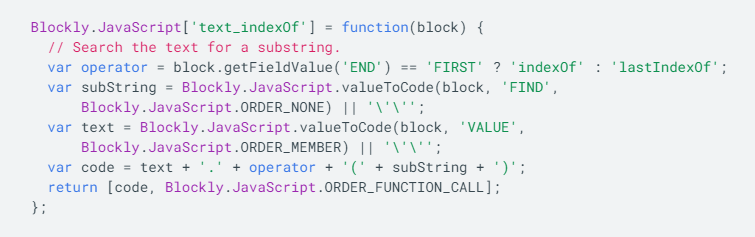
\includegraphics[scale=0.6]{img/generatingCode.png}
    \caption{Bloko kodo generatorius}
    \label{img:generatingCode}
\end{figure}

\subsubsection{Privalumai}

\begin{itemize}
    \item Eksportuojamas kodas. Vartotojai gali perkelti savo blokų programas į įprastas programavimo kalbas ir sklandžiai pereiti prie tekstinio programavimo.
    \item Atviras kodas -- visa informacija apie „Blockly“ yra atvira.
    \item Išplėčiamumas. Blokus galima modifikuoti, pridėti naujų, sričiai tinkamų arba pašalinti nereikalingus
    \item Galimybių gausa. Pasinaudojus šiuo įrankiu galima įgyvendinti sudėtingas programavimo užduotis, pavyzdžiui apskaičiuoti standartinį nuokrypį panaudojus tik vieną bloką.
    \item „Blockly“ buvo išverstas į daugiau nei 40 kalbų, įskaitant arabų ir hebrajų kalbas, kurios rašomos iš dešinės į kairę. \cite{introductionToBlockly}
    \item Sąsaja yra patraukli ir patogi vartotojui.
    \item „Blockly“ galima naudoti vien klientinėje programos dalyje, tai nereikalauja palaikymo iš serverio (nebent norima naudoti „cloud-storage“ funkciją).
    \item Veikia pagrindinėse žiniatinklio naršyklėse, įskaitant: „Chrome“, „Firefox“, „Safari“, „Opera“, „Internet Explorer“.
    \item Palaikomas „Android“ ir „iOS“ mobiliuosiuose.
\end{itemize}

\subsubsection{Trūkumai}

\begin{itemize}
    \item „Blockly“ veikia vaizdiniu formatu. Nors taip vaikams lengviau išmokti, kaip algoritmai veikia teoriniu lygmeniu, tai neišmoko tikrosios kodavimo kalbos.
    \item Tradicinės derinimo (angl. \textit{„debugging“}) galimybės yra ribotos \cite{victoria_2019}.
    \item Nėra itin daug „Blockly“ panaudojimo būdų ir variantų.
    \item Tai nėra labai populiari biblioteka, todėl internete galima ir nerasti reikiamos informacijos ar pagalbos iš kitų kūrėjų.
    \item Kalbų gausa gali trukdyti programuotojams iš skirtingų šalių komunikuoti tarpusavyje ir kurti vientisą kodą.
\end{itemize}

\subsection{„Scratch“}

„Scratch“ yra vizuali programavimo aplinka naršyklėje, leidžianti vartotojams kurti interaktyvius projektus. Ši aplinka naudoja „Blockly“ biblioteką įvariausiems projektams kurti. Vartotojai yra sukūrę daugybę projektų su „Scratch“, įskaitant animacinius filmukus, žaidimus, internetines naujienų laidas, muzikinius vaizdo įrašus, mokslo projektus, mokymo programas, simuliacijas ir kita (\ref{img:scratch} paveikslėlis).

\begin{figure}[H]
    \centering
    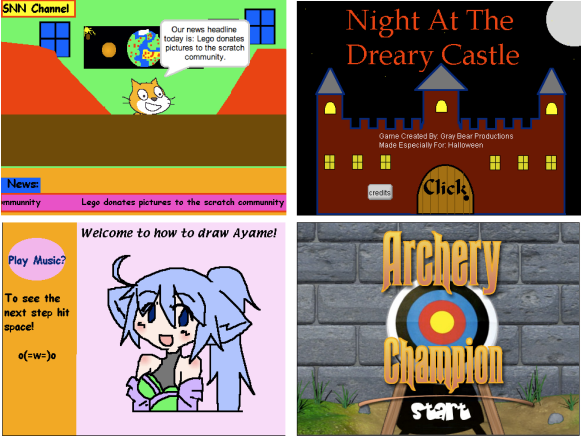
\includegraphics[scale=0.6]{img/scratch.png}
    \caption{Vartotojų sukurtų „Scratch“ projektų ekrano vaizdai, įskaitant naujienų laidą, interaktyvią istoriją, piešimo pamoką ir žaidimą.}
    \label{img:scratch}
\end{figure}

Programavimas šioje svetainėje atliekamas dėliojant spalvingus komandų blokus, kad būtų galima valdyti 2-D grafinius objektus, judančius fone, vadinamu scena. „Scratch“ projektus galima įrašyti į failų sistemą arba bendrinti „Scratch“ svetainėje.

„Scratch“ paskatino jaunus žmones mokytis tiriant ir dalijantis kartu su bendraamžiais, mažiau dėmesio skiriant tiesioginiam programavimo mokymuisi. Iš pradžių „Scratch“ buvo naudojamas neformaliojo mokymosi aplinkose, pavyzdžiui būreliuose, bibliotekose ar namuose, tačiau vis dažniau jis yra įtraukiamas ir į mokyklų veiklas.

Pagrindinis „Scratch“ tikslas yra pristatyti programavimą tiems, kurie neturi ankstesnės programavimo patirties. Šis tikslas paskatino nustatyti daugumą „Scratch“ dizaino aspektų. Kai kurie dizaino sprendimai yra akivaizdūs, pavyzdžiui, vizualinių blokų kalbos pasirinkimas, vieno lango vartotojo sąsajos išdėstymas ir minimalus komandų rinkinys. Kiti yra mažiau akivaizdūs, pavyzdžiui, kaip tikslinė auditorija paveikė tipų sistemą ir požiūrį į klaidų valdymą. \cite{maloney2010scratch}

\section{„Blockly“ ir „Jetbains MPS“ įrankių palyginimas}
% https://confluence.jetbrains.com/display/MPS/MPS+publications+page

\begin{table}[h]
\begin{tabular}{|l|c|c|}
\hline
\textbf{}                                                                                  & \textbf{„Blockly“}                                                                                                                                    & \textbf{„MPS“}                                                                                                                                                                        \\ \hline
\textbf{DSL atvaizdavimas}                                                                 & Blokinis                                                                                                                                              & Tekstinis/Lentelių                                                                                                                                                                             \\ \hline
\textbf{Kalba}                                                                             & \begin{tabular}[c]{@{}c@{}}JavaScript, Lua, Dart,\\ Python, PHP ir kitos\end{tabular}                                                                 & \begin{tabular}[c]{@{}c@{}}Be papildomų įskiepių tik\\ Java, XML ir Ant\end{tabular}                                                                                                           \\ \hline
\textbf{Prieinamumas internete}                                                            & Prieinama                                                                                                                                                     & -                                                                                                                                                                                              \\ \hline
\textbf{IDE}                                                                               & \begin{tabular}[c]{@{}c@{}}Galima naudoti bet kokį\\ pasirinktą kodo redaktorių\end{tabular}                                                          & \begin{tabular}[c]{@{}c@{}}Veikia „IntelliJ IDEA“ su „MPS“ \\ įskiepiu arba „JetBrains MPS“ \\ programose\end{tabular}                                                                         \\ \hline
\textbf{\begin{tabular}[c]{@{}l@{}}Naujų kalbos sąvokų\\ kūrimo sudėtingumas\end{tabular}} & \begin{tabular}[c]{@{}c@{}}Nesunku, ypač naudojantis\\ „Blockly Developer Tools“\end{tabular}                                                         & \begin{tabular}[c]{@{}c@{}}Ganėtinai sudėtinga, nes reikia \\ rankiniu būdu aprašyti struktūrą,\\ apribojimus, elgesį ir kt.\end{tabular}                                                      \\ \hline
\textbf{Redagavimas}                                                                       & Laisva forma                                                                                                                                          & Projekcinis                                                                                                                                                                                    \\ \hline
\textbf{Įdiegimo sudėtingumas}                                                             & \begin{tabular}[c]{@{}c@{}}Vartotojui nieko diegti nereikia,\\ o programuotojams įdiegti\\  „Blockly“ į savo projektą \\ nėra sudėtinga\end{tabular}  & \begin{tabular}[c]{@{}c@{}}Ir vartotojams, ir programuotojams\\ reikia atsisiųsti IDE -- nėra labai\\ patogu.\end{tabular}                                                                      \\ \hline
\textbf{\begin{tabular}[c]{@{}l@{}}Programos paleidimo\\ sudėtingumas\end{tabular}}        & \begin{tabular}[c]{@{}c@{}}Programuotojui pakanka \\ išsaugoti kodo failą, o vartotojui \\ tereikia paspausti vieną \\ paleidimo mygtuką\end{tabular} & \begin{tabular}[c]{@{}c@{}}Gana sudėtinga, nes reikia\\ ir iš naujo sukompiliuoti \\ sukurtą kalbą, ir žinoti, kaip \\ paleisti pačią programą. Tam reikia \\ papildomai domėtis.\end{tabular} \\ \hline
\end{tabular}
\end{table}

Remiantis šių įrankių palyginimu, galima nuspręsti, kuris iš jų yra patogesnis tiek galutiniam vartotojui, tiek programuotojams, bei tinkamesnis norint kurti edukacinį turinį. Atsižvelgiant į tai, jog „Blockly“ naudoja blokinį DSL savokų atvaizdavimą ir yra lengvai prieinamas internete --  nei vartotojams, nei programuotojams nereikia siųstis papildomų programų -- taip pat nėra sunku paleisti programą, „Blockly“ yra patogesnis besimokantiems vartotojams. „JetBrains MPS“ reikalauja papildomų priemonių ir žinių norint tiek kurti naujas metakalbas, tiek jas paleisti ar eksportuoti.

Naujų specializuotųjų kalbų kūrėjams taip pat gali būti patogiau naudoti būtent „Blockly“, nes yra gana paprasta sukurti naujas kalbų sąvokas, nereikia apibrėžti jų požymių taip sudėtingai, kaip reikia tai daryti naudojant „JetBrains MPS“. Taip pat „Blockly“ palaiko žymiai daugiau programavimo kalbų, todėl jis yra universalesnis, pritaikytas didesnei grupei skirtingų domenų, programuotojai turi daugiau pasirinkimo laisvės renkantis, kuria kalba rašyti programas.

\section{Meta kalbų nauda kuriant edukacinius žaidimus}

Šiame skyrelyje apžvelgiama meta kalbų nauda kuriant edukacinius žaidimus.
\subsection{Redaktorius}
Kadangi specializuotąsias kalbas bei jų kūrimo įrankius gali naudoti ne tik programuotojai, bet ir daug programavimo žinių neturintys žmonės, pavyzdžiui, mokytojai, reikia, kad jie neišsigąstų programų ar įrankių sudėtingumo. Todėl, kur įmanoma, kalbai ir jos sąvokoms turėtų būti naudojamos žinomos ar lengvai išmokstamos abstrakcijos ir žymėjimai. Taip pat svarbu išlaikyti gerą kodo bei sąvokų skaitomumą. Dauguma specializuotųjų kalbų naudoja priemones, kurios padeda sukurti patrauklesnius redaktorius.

\subsection{Laiko taupymas}

Rimta problema įprastiniame programavime yra ta, jog gali praeiti daug laiko tarp žinojimo, kokius principus pritaikyti norint išspręsti problemą, ir sėkmingo sprendimo užrašymo programinio kodo pavidalu. Kartais įmanoma paaiškinti problemą ir sprendimą jai per kelias minutes ar valandas, bet to sprendimo užrašymas kodu užtrunka žymiai ilgiau. Taip yra todėl, kad žmonės tarpusavyje bendrauja natūralia kalba, kurios žodynas yra turtingesnis, o komunikuojant kodu reikia naudoti bendrosios paskirties programavimo kalbas -- šios kalbos yra žymiai mažiau išraiškingos. Taigi, tam, kad žmogus paaiškintų programą/problemą kitam, tai padaryti įmanoma vien pasinaudojus aukšto lygio (angl. \textit{„high-level“}) idėjomis.

Specializuotosios kalbos gali padėti sutrumpinti laiko tarpą nuo idėjos sugalvojimo iki jos įgyvendinimo dėl to, kad yra naudojamos abstrakčios sąvokos, panašios į OOD (angl. \textit{Object-oriented design}) proceso. Žinoma, tam, kad būtų sutaupyta laiko, reikia, kad vartotojas būtų susipažinęs su specializuotomis kalbomis ir naudojamu įrankiu.

\subsubsection{Kodo eilučių kiekio sumažinimas}

Vienas svarbiausių DSL naudojimo pranašumų yra tas, kad darbas DSL apimamoje programinės įrangos kūrimo srityje yra daug efektyvesnis vien todėl, kad nereikia daryti didelės dalies monotoninio darbo rankiniu būdu. Kai DSL programos šaltinio kodas yra generuojamas, galima naudoti gražias, sričiai būdingas abstrakcijas, kadangi generatorius, kaip ir kompiliatorius, gali pašalinti abstrakcijas ir generuoti optimalų kodą, taigi galima žymiai sumažinti rašomų kodo eilučių skaičių ir taip pat sutaupyti laiko programuotojams.

\subsection{Retesnės klaidos}

DSL naudojimas gali pagerinti sukurto produkto kokybę: mažiau klaidų, geresnis architektūrinė atitiktis, padidėjęs techninės priežiūros efektyvumas. Taip būna pašalinus (nereikalingus) laisvės lygius, kodo dubliavimąsi ir automatizavus pasikartojančius rankinius darbus.

Tai svarbu atsižvelgiant į tai, jog į kalbos bei programos kūrimą gali būti įtraukti ir ne programuotojai, o ir tam tikros srities specialistai. DSL naudojimas sumažina tikimybę, kad vykdant kodą atsiras naujų klaidų. 

\subsection{Kūrėjai ir srities specialistai}

Kadangi kuriant DSL programuotojams reikia glaudžiai bendradarbiauti su tos srities specialistais, patys kūrėjai gali išmokti kažko naujo, o srities specialistai geriau suprasti, su kokiomis problemomis susiduria IT specialistai.

Kai DSL sritis yra švietimas arba edukaciniai žaidimai, tai reiškia, jog yra suteikiama galimybė mokytojams, mokiniams ar studentams įsitraukti į žaidimo kūrimo procesą, pvz.: sugalvoti naujas užduočių idėjas žaidime ir t.t.

\section{Taikymas}

Šiame skyriuje aprašomi sukurti du edukaciniai žaidimai, naudojantys specializuotąsias kalbas. Pirmasis projektas buvo sukurtas metais anksčiau, bet yra svarbus norint parodyti „JetBrains MPS“ galimybes. Antrasis projektas sukurtas norint palyginti skirtingus įrankius, bei išsiaiškinti, ar „Blockly“ gali būti patogesnis naudoti tiek programuotojams, tiek mokiniams ir mokytojams.

\subsection{„JetBrains MPS“ projektas}

Šio projekto tikslas buvo sukurti specializuotąsias kalbas skirtas edukaciniam žaidimui, kuris padėtų mokytis matematikos (žr. Priedas nr. 1).
Žaidimo ir domeno kalbų kūrimui buvo naudotas „JetBrains MPS“ įrankis bei „jMonkeyEngine“ atviro kodo žaidimų variklis (angl. \textit{game engine}). „jMonkeyEngine“ -- variklis, sukurtas Java kalbos pagrindu, todėl jį galima nesunkiai įterpti į MPS projektą, kadangi MPS taip pat yra paremtas Java kalba.

Sukurtas edukacinis žaidimas padeda mokytis daugybos lentelės ar kitokių ne pernelyg sudėtingų matematinių skaičiavimų. Žaidimo veikėjas yra vaikščiojantis „trolis“, einantis labirintu, kurį yra apibrėžęs vartotojas, ir kas kelis metrus šiam veikėjui yra užduodami matematiniai klausimai (\ref{img:galutinisProjektas} paveikslėlis).

Programos vartotojas MPS redaktoriuje turi nurodyti:
\begin{enumerate}
\item žaidimo pasaulio matmenis (ilgį ir plotį),
\item taškų kiekį, suteikiamą už gerai atsakytą klausimą,
\item pradinį gyvybių skaičių,
\item „true“ prie veikėjo sukūrimo sakinio, jei norima jį sukurti,
\item labirinto sienų, nurodytomis x ir z vertėmis, sąrašą,
\item daugybos lentelės ar kitokių matematinių klausimų sąrašą, pvz.: 4*8.
\end{enumerate}

\begin{figure}[H]
    \centering
    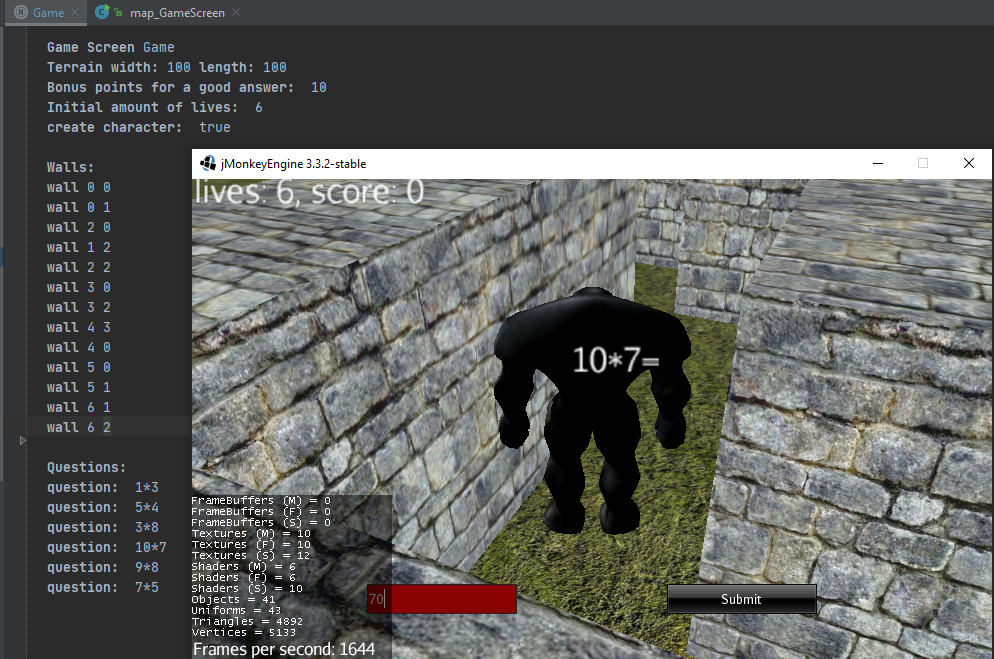
\includegraphics[scale=0.5]{img/galutinisProjektas.png}
    \caption{„JetBrains MPS“ edukacinis žaidimas ir jo redaktorius(kairėje)}
    \label{img:galutinisProjektas}
\end{figure}

Projektas yra sudarytas iš trijų specializuotųjų kalbų: \textit{„Engine“}, \textit{„FeedbackLang“}, ir \textit{„MathTaskLang“}. MPS kalbos gali lengvai naudoti viena kitą.

\subsubsection{Žaidimo kalbos sąvokos}

DSL kūrimas prasideda nuo jo sąvokų apibrėžimo, nes MPS sąvokos/koncepcijos yra apibrėžimai, apibūdinantys abstrakčią DSL sintaksės elemento struktūrą. Toliau bus aprašytos sąvokos, kurių prireikė žaidime.

Esminės žaidimo sąvokos aprašytos „Engine“ kalboje:
\begin{itemize}
\item „MainCharacter“ arba „pagrindinis veikėjas“: ši sąvoka turi vieną savybę -- „created“, kuri yra loginio tipo ir reiškia, kad veikėjas yra sukuriamas, jei savybei priskirta būsena „true“.
\item „TerrainSize“ arba „pasaulio dydis“ su ilgio ir pločio savybėmis.
\item „Wall“ arba „sienos“ koncepcija apibūdina statomą labirinto sieną, kuri turi savybes „x-value“ bei „z-value“. 
\item „GameScreen“ arba „žaidimo ekranas“: ši sąvoka apibūdina viso žaidimo struktūrą, ji turi tokius vaikinius mazgus kaip: „TerrainSize“, „Wall“, „MainCharacter“, „Lives“, „Score“, bei „Questions“. Galima kurti atskirus „GameScreen“ atvejus.
\end{itemize}

„FeedbackLang“ arba „grįžtamojo ryšio“ kalboje sukurtos šios sąvokos:
\begin{itemize}
    \item „Lives“ arba „gyvybės“ -- ši sąvoka turi savybę „initialLives“ arba „pradinės gyvybės“ ir ji leidžia žinoti kiek gyvybių žaidėjui yra likę.
    \item „Score“ arba „taškai“ su savybe „bonus“ nurodo kiek taškų bus pridedama už teisingai atsakytą klausimą.
\end{itemize}

Matematinių klausimų sąvokos apibrėžtos kalboje „MathTaskLang“:
\begin{itemize}
    \item „Question“ arba „klausimo“ sąvoka su savybe „task“ apibūdina atskirą matematinį uždavinį
    \item „Questions“ sąvoka turi vaiko mazgą „Question“, todėl ši sąvoka saugo matematinių uždavinių sąrašą.
\end{itemize}

\subsubsection{Kodo generavimas ir paleidimas}
Norint paleisti šį žaidimą, būtinas vykdomasis kodas, kuris sukuriamas kodo generatorių. Vartotojui redaktoriuje sukūrus ir apibrėžus sąvokas, kiekvienai kalbų sąvokai, kuri nėra šakninė, yra pritaikomos redukcijos taisyklės, o šios panaudojamos generuojant galutinį Java kalbos kodą.

\subsection{„Blockly“ projektas}

Remiantis ankstesniu „Blockly“ ir „Jetbains MPS“ įrankių palyginimu, galima matyti, jog nors MPS palaiko lenteles ir diagramas, ji daugiausia skirta kurti tekstines kalbas, o tai nėra taip patogu vaikams ir paaugliams norintiems išmokti programuoti arba kitų disciplinų.

Šiam darbui buvo sukurtas edukacinis žaidimas, kurio tikslas -- mokyti vaikus ir jaunus paauglius programavimo pagrindų, matematikos ir kitų disciplinų. Žaidimas paremtas anksčiau aprašytu labirinto žaidimu, tačiau „Blockly“ versijoje pridėta daugiau skirtingų užduočių ir yra mokoma programavimo, taigi yra pridėta edukacinės vertės žaidimui (žr. Priedas nr. 2).

Šiam projektui buvo naudota „Blockly“ biblioteka JavaScript aplinkai. Žaidimas parašytas HTML, CSS ir JavaScript kalbomis, todėl jis veikia naršyklėje. Jis susideda iš aštuonių iš anksto apibrėžtų lygių, bei papildomų lygių, kuriuos galima generuoti automatiškai. Projekto esmė yra dėliojant judėjimo/loginius blokelius pereiti labirintą ir keliaujant teisingai atsakyti į užduodamus klausimus (\ref{img:blocklyGame} paveikslėlis). Už gerai atsakytą klausimą arba pereitą lygį suteikiamas vienas taškas vartotojui. Blokams naudojamas \ref{section:dazniausiStiliai} skyriuje aprašytas natūralios kalbos stilius, nes žaidimas yra skirtas vidurinių mokyklų mokiniams, o šiuo stiliumi galima supaprastintai apibrėžti pagrindinius programavimo principus.

\begin{figure}[H]
\centering
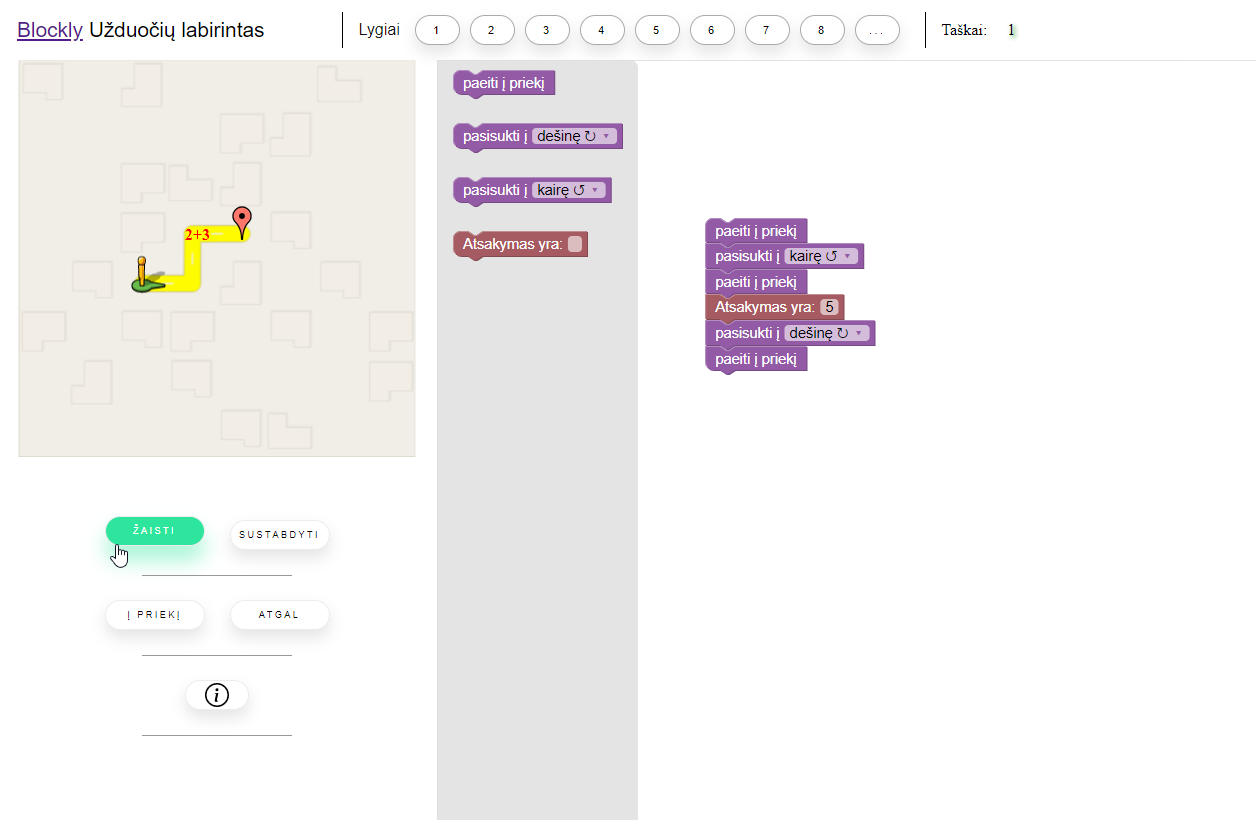
\includegraphics[scale=0.4]{img/gameView.png}
\caption{Žaidimo vaizdas su pirmojo lygio teisingai sudėliotais blokais}
\label{img:blocklyGame}
\end{figure}

\subsubsection{Žaidimo kalbos sąvokos}

Šio mokomojo žaidimo kalbos sąvokos yra atvaizduojamos grafiniai blokais, kuriuos vartotojas gali dėlioti ekrane. Kadangi žaidimas moko programavimo pagrindų, dauguma blokų atitinka programavime vartojamus terminus:
\begin{itemize}
    \item Blokas „Paeiti į priekį“ apibūdina sąvoką, kuri leidžia žaidimo veikėjui paeiti vienu laukeliu į priekį ta kryptimi, į kurią yra žiūrima.
    \item „Pasisukti į \_“ blokelis turi pasirinkimus, kurie leidžia nustatyti į kurią pusę, kairę ar dešinę, veikėjui pasisukti.
    \item „Atsakymas yra \_“ objektas turi įvesties lauką, kuriame nurodomas manomas teisingas atsakymas. Atsakymas gali būti tiek tekstinis, tiek skaitinis. Šis blokas turi būti padėtas tik toje blokų grandinės dalyje, kur manoma, jog veikėjas bus atsistojęs ant klausimo laukelio labirinte.
    \item Blokas „Kartojant iki finišo vykdyti: \_“ yra ciklo „while“ atitikmuo leidžiantis vykdyti tam tikrus veiksmus iki tol, kol bus pasiektas finišas. Tai šakninis mazgas, todėl jam reikia pridėti vaikų mazgus, kad jis veiktų tinkamai.
    \item „Jei kelias \_ tuomet \_“ blokas yra sąlyginės operacijos „if“ atitikmuo, kuriam reikia nurodyti sąlygą, išrinktą iš pasirinkimų („egzistuoja priekyje“, „eina į dešinę ↻“, „eina į kairę ↺“, „turi užduotį“), bei veiksmus kurie bus įgyvendinti, jei sąlyga bus patenkinta. Pasirinkimas „egzistuoja priekyje“ patikrina, ar ta kryptimi, kuria yra stovima, yra kelias priekyje; „eina į dešinę ↻“ ir „eina į kairę ↺“ pasirinkimai tikrina, ar, žiūrint nuo veikėjo esamos padėties, yra kelias kairėje arba dešinėje; „turi užduotį“ pasirinkimas grąžina teigiamą atsaką, jei žaidimo veikėjo koordinatė sutampa su užduoties koordinate labirinte.
    \item „Jei kelias \_ tuomet \_, kitu atveju \_“ sąvoka yra panaši į „if else“ salyginę operaciją, kuriai reikia parinkti sąlyga iš sąrašo (sąlygų variantai yra tokie patys kaip ir „Jei kelias \_ tuomet \_“ sąvokai), veiksmus kurie bus įgyvendinti, jei sąlyga bus patenkinta, arba ne.
\end{itemize}

Norint pereiti lygį reikia teisinga tvarka sudėlioti blokelius, paspausti mygtuką „Žaisti“ -- tuomet veikėjo figūra pradeda vaikščioti labirintu ir, jei blokeliai buvo sudėti tinkamai, yra pasiekiamas finišas ir ekrane gaunamas sveikinimo pranešimas. Jei „atsakymo“ blokelis yra padėtas netinkamoje vietoje, paleidus programą apie tai yra pranešama tuomet, kai yra pasiekta jo vykdymo eilė.

\subsubsection{Automatiškai generuojami lygiai}

Žaidime yra galimybė automatiškai generuoti lygius su nauju išdėstymu ir klausimais. Vartotojas turi pasirinkti, per kiek blokelių yra norima įveikti labirintą, ir pagal šį skaičių generuojami labirintai. Kai kurie sukurti lygiai turi matematines užduotis, kai kurie iš jų neturi, taip pat skirtinguose lygiuose gali skirtis ir pasirenkamų blokelių tipai -- nepaisant to, visi atitinka pradžioje pasirinktą blokelių skaičių (\ref{img:randomLevelGame} paveikslėlis).

\begin{figure}[H]
\centering
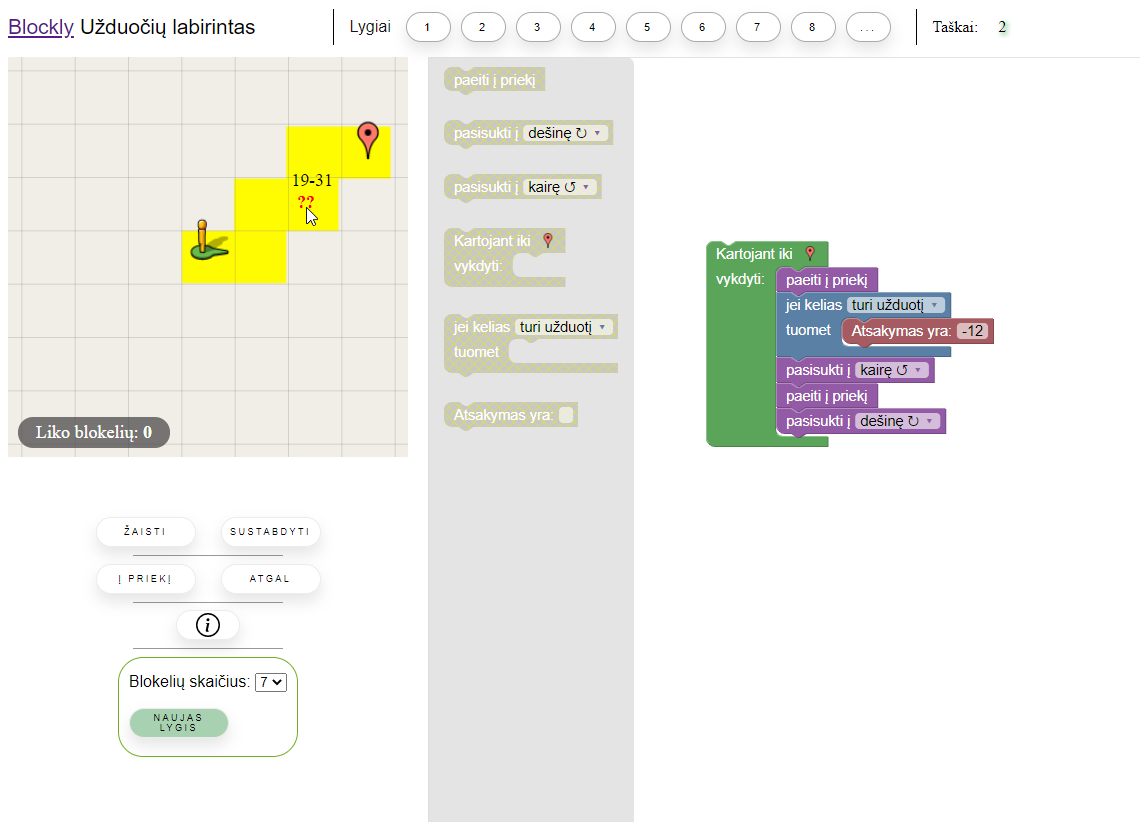
\includegraphics[scale=0.4]{img/randomLevelGame.png}
\caption{Sugeneruotas 7-ių blokelių lygis su užduotimi ir jo sprendimas}
\label{img:randomLevelGame}
\end{figure}

\subsubsection{Žaidimų kūrimo principų atitikimas}
Mokomasis žaidimas buvo išbandytas keleto 5 klasės mokinių, todėl jį kuriant buvo atsižvelgta į 2.2 skyriuje minėtus principus, apibrėžiančius puikius edukacinius žaidimus: 
\begin{itemize}
    \item Nustatyti aiškūs tikslai ir instrukcijos -- svetainėje galima matyti žaidimo taisykles (\ref{img:info} paveikslėlis), o jo tikslas yra teisingai atsakyti į užduotus klausimus ir padėti veikėjui pasiekti finišo koordinatę.
        \begin{figure}[H]
        \centering
        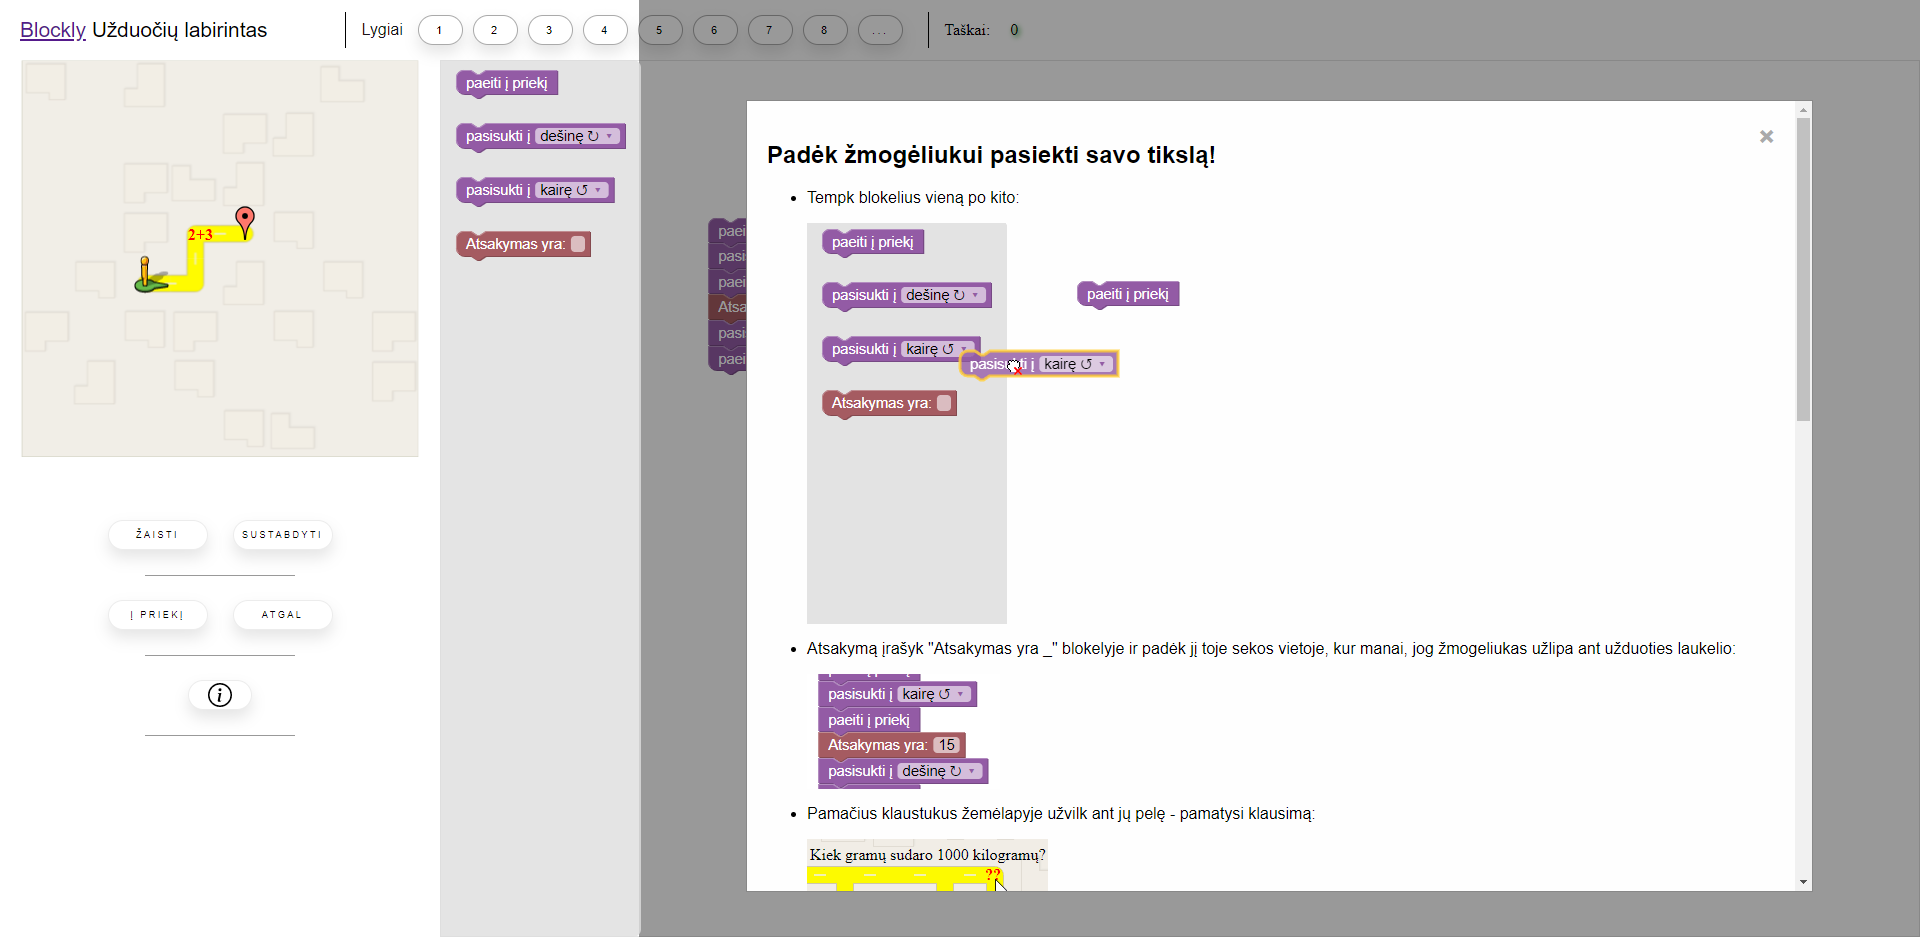
\includegraphics[scale=0.3]{img/info.png}
        \caption{Žaidimo taisyklių vaizdas svetainėje}
        \label{img:info}
        \end{figure}
    \item Žaidėjo įtraukimas per veikėjus ir istoriją -- vartotojas žaidime valdo žmogeliuką, kuriam reikia pasiekti finišą, jis eina tarsi atgal namo per kelius apsuptus kitų gyvenamųjų namų.
    \item Vertinimo įtraukimas į žaidimo eigą -- paspaudus paleidimo mygtuką, iškart yra vertinama, ar blokeliai buvo sudėti tinkamai ir yra pranešama apie klaidas, jei tokių būta.
    \item Vidinė ir išorinė motyvacija -- puikiai perėjus lygį arba teisingai atsakius į klausimus, yra suteikiami taškai.
    \item Autonomijos palaikymas -- kai kuriuose lygiuose žaidėjui yra suteikta galimybė naudoti bet kiek ir bet kokių blokelių, todėl jis gali pasirinkti blokelių dėliojimo sudėtingumą. Septintajame lygyje yra dvi užduotys, bet viena iš jų yra neprivaloma, tai reiškia, kad žaidėjas gali nuspręsti bandyti įveikti neprivalomą užduotį, arba ne (\ref{img:neprivaloma} paveikslėlis). Už šios užduoties įveikimą skiriamas papildomas taškas.
        \begin{figure}[H]
        \centering
        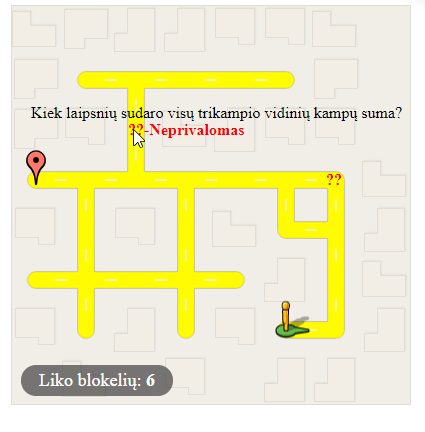
\includegraphics[scale=0.5]{img/septintaUzd.png}
        \caption{Septintasis lygis su viena neprivalomi užduotimi}
        \label{img:neprivaloma}
        \end{figure}
    \item Bendrystės skatinimas -- šiame žaidime nėra jokio aiškaus skatinimo bendradarbiauti, palikta rinkimosi laisvė mokiniams -- jie gali konsultuotis su mokytojais arba kitais mokiniais, arba gali spręsti uždavinius patys.
    \item Kompetencijos palaikymas -- kiekvienas lygis yra šiek tiek sudėtingesnis, nei praeitas, arba jie išmoko naudotis naujomis sąvokomis, pavyzdžiui trečiame lygyje reikia panaudoti šešis blokelius, o ketvirtame jau septynis.
    \item Produktyvios nesėkmės -- žaidėjui netinkamai sudėjus blokelius, apie klaidą yra pranešama ir ta patį lygį bandyti paleisti ir pereiti galima nelimituotą kiekį kartų.
    \item Skatinimas tyrinėti -- vartotojas gali ilgą laiką sukti galvą dėl to, kaip išspręsti ypač tolesnius lygius.
    \item Praktika -- panašios užduotys ir jų atkartojimas padeda geriau įsiminti jų sprendimo būdus. Šiame žaidime galima automatiškai generuoti lygius, pagal blokelių skaičių, dėl to dauguma labirintų gali atrodyti panašūs pasirinkus tą patį blokelių skaičių jiems visiems.
\end{itemize}

\subsubsection{Tyrimas}
% kaip kas
Sukurtas edukacinis žaidimas (su iš anksto nustatytais lygiais, be automatinio lygių generavimo) buvo išbandytas 56-ių penktos klasės „Ąžuolyno“ progimnazijos mokinių. Visi dalyviai užpildė apklausą apie šio žaidimo naudą. Mokiniams buvo parodytas informacinis vaizdo įrašas (žr. Priedas nr. 3), kuriame paaiškinama, kaip naudotis WEB programa, kaip dėlioti blokelius ir paleisti žaidimą, taip pat už ką gaunami taškai. 

Dauguma mokinių perėjo 3-4 lygius (\ref{img:pereitiLygiai} paveikslėlis), būtent tuose lygiuose įvedamas „while“ tipo blokas, kurį pradžiamoksliams yra sudėtingiau suprasti, nei paprastas ėjimo ar sukimosi operacijas. Nemažai mokinių perėjo ir 5-6 lygius, todėl galima teigti, jog kai kurie yra išmokę „while“ ir „if“ operacijų konceptus. 7-8 lygius perėjo didesnis procentas apklaustųjų, nei 0-2 lygius, reiškia žaidimas buvo gana suprantamas ir įveikiamas.

\begin{figure}[H]
\centering
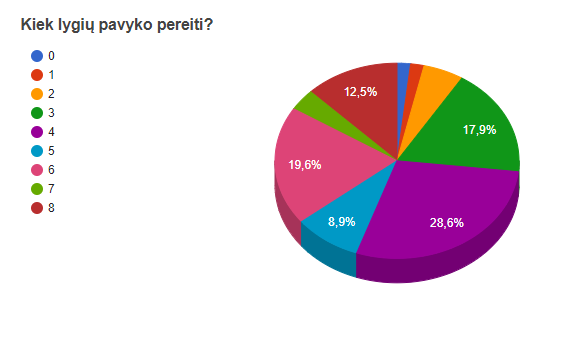
\includegraphics[scale=0.8]{img/lygiuPerejimas.png}
\caption{Mokinių pereitų lygių statistika}
\label{img:pereitiLygiai}
\end{figure}

69,6\% respondentų paklausti, ar toks edukacinis žaidimas atrodo įdomiau nei paprastas tekstinis programavimas, atsakė teigiamai (\ref{img:susidomejimas} paveikslėlis), tiesa, keletas mokinių paliko komentarą, jog programa „Scratch“ (sukurta naudojantis „Blockly“ biblioteka) jiems patinka dar labiau. Deja 62,5\% apklaustųjų atsakė, jog žaisdami neišmoko nieko naujo (\ref{img:arSuzinojai} paveikslėlis), nepaisant to tikimasi, jog jie bent jau pasikartojo turimas žinias. Taip pat tik 12,5\% mokinių atsakė, jog žaistų tokį žaidimą po pamokų (\ref{img:arZaistum} paveikslėlis).

\begin{figure}[H]
\centering
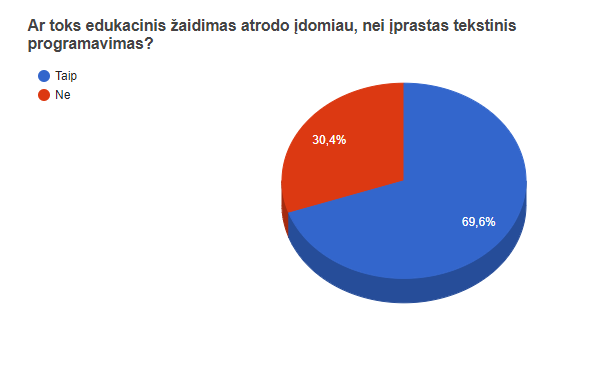
\includegraphics[scale=0.8]{img/idomiauNei.png}
\caption{Mokinių susidomėjimas edukaciniu žaidimu, lyginant su įprastu programavimu}
\label{img:susidomejimas}
\end{figure}

\begin{figure}[H]
\centering
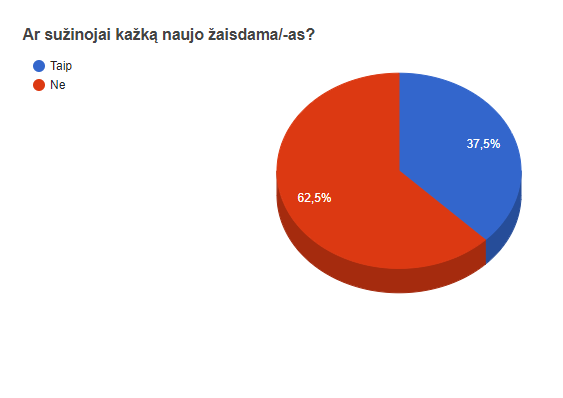
\includegraphics[scale=0.8]{img/arSuzinojai.png}
\caption{Mokinių nuomonė apie edukacinę žaidimo vertę}
\label{img:arSuzinojai}
\end{figure}

\begin{figure}[H]
\centering
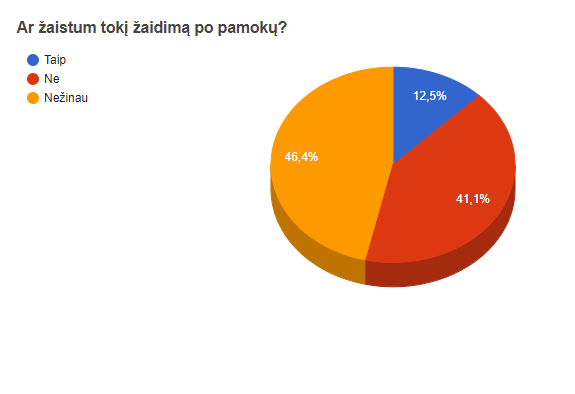
\includegraphics[scale=0.8]{img/arZaistum.png}
\caption{Respondentų atsakas, paklausus ar žaistų tokį žaidimą po pamokų}
\label{img:arZaistum}
\end{figure}

Mokiniai galėjo įvertini lygių sudėtingumą skalėje nuo 0 iki 100 -- šimtas reikštų, kad lygiai neišsprendžiamai sudėtingi. Daugumai moksleivių lygiai buvo vidutiniškai sunkūs (\ref{img:lygiuSudetingumas} paveikslėlis). Prie šio rezultato gavimo galėjo prisidėti tai, kad buvo sukurtas informacinis vaizdo įrašas, kuriame paaiškinamos žaidimo taisyklės ir, pagal apklausos rezultatus, apie 70\% žmonių buvo bent ganėtinai aišku, kaip naudotis sistema ir koks yra žaidimo tikslas (\ref{img:arAisku} paveikslėlis).

\begin{figure}[H]
\centering
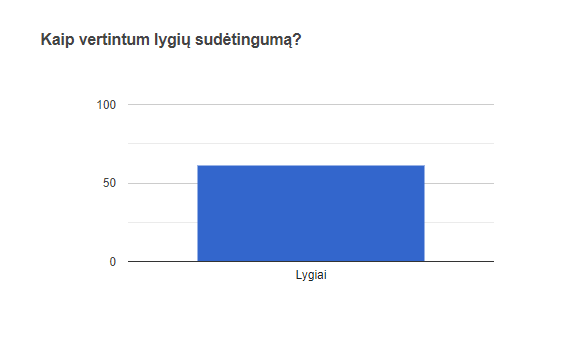
\includegraphics[scale=0.8]{img/sudetingumas.png}
\caption{Lygių sudėtingumo vidurkis}
\label{img:lygiuSudetingumas}
\end{figure}

\begin{figure}[H]
\centering
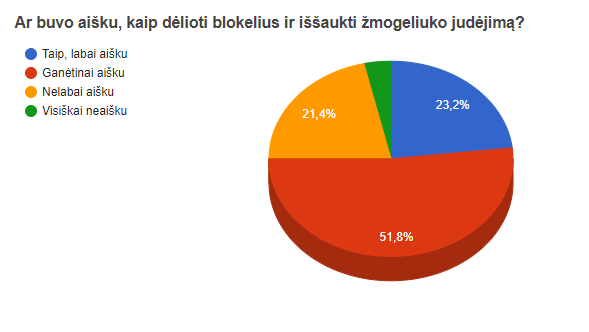
\includegraphics[scale=0.8]{img/arAisku.png}
\caption{Žaidimo valdymo patogumas}
\label{img:arAisku}
\end{figure}

Kadangi informacinės technologijos įsilieja į vis daugiau sričių ir programuotojų reikia vis daugiau, buvo norima sužinoti, ar mokykloje įgytos žinios yra pakankamos norint išspręsti užduotis šiame žaidime. Iš apklausos rezultatų galima matyti, jog didžiajai daugumai įgytos žinios padėjo, arba jie nėra tikri, kaip atsakyti į šį klausimą (\ref{img:arZiniosPadejo} paveikslėlis).

\begin{figure}[H]
\centering
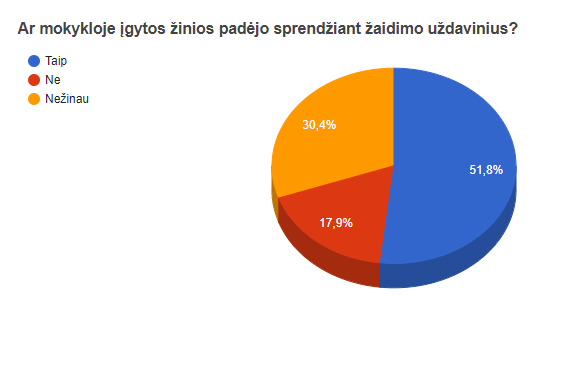
\includegraphics[scale=0.8]{img/arZiniosPadejo.png}
\caption{Mokykloje įgytų žinių pagalba žaidime}
\label{img:arZiniosPadejo}
\end{figure}

\sectionnonum{Rezultatai ir išvados}
Šiame darbe nagrinėtos metakalbos, metaprogramavimas ir jų pavyzdžiai. Apibrėžti puikių edukacinių žaidimų kūrimo principai ir apžvelgtas jų gebėjimas įtraukti žmones į mokymosi procesą.

Nagrinėti „JetBrains MPS“ ir „Blockly“ specializuotųjų kalbų kūrimo įrankiai, palygintos jų stipriosios ir silpnosios pusės. Šiam darbui sukurtas edukacinis žaidimas, naudojantis „Blockly“ biblioteka ir kalbomis, jis palygintas su panašios tematikos mokomuoju žaidimu, paremtu „JetBrains MPS“ aplinka. Remiantis atlikta mokinių apklausa ir patirtimi kuriant edukacinius žaidimus, suformuoti meta kalbų kuriant edukacinius žaidimus privalumai:
\begin{itemize}
    \item Meta kalbų abstrakcijos ir sąvokos padeda taupyti laiką, nes šios kalbos padeda sumažinti monotoninio darbo kiekį, kas padeda sumažinti kodo eilučių skaičių. Metakalbos gali padėti kontroliuoti kuriamo projekto sudėtingumą, tai yra, padaryti jį skaitomesniu ir patogesniu naudoti. 
    \item DSL naudojimas gali pagerinti produkto kokybę, daroma mačiau klaidų.
    \item Pradedant mokytis programavimo yra svarbu pirmiau išmokti programavimo principų, o juos aiškiau leidžia paaiškinti vizualiosios kalbos ir jų DSL.
    \item Specializuotosios kalbos leidžia srities specialistams ir vartotojams labiau įsilieti į žaidimo kūrimą, o tai gali padėti geriau suprasti tą sritį, bei įtraukti daugiau naudingų idėjų į projekto kūrimo procesą.
\end{itemize}

Apibendrinus darbo rezultatus (surinktą informaciją, sukurtą edukacinio žaidimo projektą bei apklausą) galima suformuluoti tokias išvadas:
\begin{itemize}
    \item Technologijos -- svarbus kasdienio žmogaus gyvenimo aspektas, todėl ateities švietimo sistema taip pat turi keistis kartu su technologijomis. Edukaciniai žaidimai turėtų būti ateities švietimo proceso dalis, kadangi manoma, jog tokie žaidimai gali padidinti moksleivių motyvaciją mokytis, pagerinti socialinius įgūdžius ir kt.
    \item Tam, kad edukaciniai žaidimai taptų populiaresni, norisi turėti įvairesnius būdus ir instrumentus jiems kurti. DSL panaudojimas ir atitinkami instrumentai gali išplėsti edukacinių žaidimų sritį ir labiau įtraukti moksleivius į mokymosi procesą.
    \item MPS gali būti tinkamas įrankis kurti edukacinius žaidimus paaugliams ir labiau programavime patyrusiems mokytojams/dėstytojams, nes nėra lengva priprasti prie MPS redaktoriaus, o laikas kuriant kalbas yra sutaupomas tik tuomet, kai kūrėjas yra susipažinęs su šia sistema.
    
    „Blockly“ yra labiau pritaikytas jaunesniems vaikams, taip pat juo naudotis ir kurti kalbas yra patogiau, kadangi nereikia siųstis specialaus IDE, programas galima pasiekti naršyklėje ir kalbų generatorius galima rašyti bet kokia pasirinkta programavimo kalba.
    \item Apklausa parodė, jog mokiniams žymiai įdomiau mokytis programavimo ar kitų dalykų interaktyviai, žaidžiant. Dauguma apklausos dalyvių atsakė, jog taip mokytis įdomiau, nei iškart mokytis tekstinio programavimo.
    \item Sukurtas žaidimo projektas galbūt buvo per sudėtingas 5-tos klasės mokiniams, nes dauguma neišsprendė visų aštuonių lygių, nors daugumai buvo aišku, kaip valdyti žaidimą ir kokie yra jo tikslai. 
    \item Deja tik septyni apklaustieji nurodė, jog žaistų tokį žaidimą po pamokų, taigi tai reiškia, jog sukurtą projektą dar galima tobulinti, pridėti įdomesnių užduočių ir interaktyvumo. Galima būtų labiau įtraukti vartotojus į žaidimo istoriją ir veikėjus, gražiau apipavidalinus projektą, sukūrus žaidimui istoriją ar sukūrus galimybę varžytis/bendradarbiauti su kitais mokiniais. Taip pat įmanoma sužadinti daugiau motyvacijos mokiniams leidžiant kažką gauti už surinktus taškus žaidime, pavyzdžiui: už taškus galima būtų nusipirkti naują veikėjo išvaizdą. Tam, kad žaidimas neatrodytų pernelyg sudėtingas, galima būtų įterpti užuominas padedančias pereiti lygius, arba galimybę šias užuominas nusipirkti už surinktus taškus.
\end{itemize}

\printbibliography[heading=bibintoc]  

\sectionnonum{Sąvokų apibrėžimai}

\textbf{Ludologija (angl. \textit{„Ludology“})} -- žaidimų studijos, kurių tyrimo objektai yra žaidimai, į juos įtraukiami žaidėjai ir jų kultūra.\cite{frasca1999ludology}

\textbf{Specializuota kalba / meta kalba} -- specialios paskirties kalba, kurios priemonėmis aprašoma kuri nors kita kalba.

\textbf{Metakalbos} -- specialios paskirties kalbos, kurių priemonėmis aprašoma kuri nors kita kalba.

\textbf{Metaprogramavimas} -- programavimas susijęs su metakalbomis.

\textbf{Edukaciniai žaidimai} -- žaidimai, specialiai sukurti švietimo tikslais arba turintys ugdomąją vertę.

\textbf{MPS} -- „JetBrains“ sukurtas įrankis skirtas į kalbą orientuotam programavimui (angl. \textit{„MetaProgrammingSystem“}).

\textbf{Žaidimų variklis} --  programinės įrangos sistema, skirta kompiuterinių žaidimų kūrimui ir plėtojimui.

\textbf{„jMonkeyEngine“} -- žaidimų variklis, specialiai sukurtas moderniam 3D kūrimui, nes jame plačiai naudojama šešėlių technologija. Naudojant šį variklį 3D žaidimus galima kurti tiek „Android“ įrenginiams, tiek kompiuteriams.

\sectionnonum{Santrumpos}

\textbf{DSL} -- kalba, specializuota tam tikroje taikymo srityje (angl.\textit{ domain-specific language}).

\textbf{GPL} -- bendrosios paskirties kalba (angl.\textit{general-purpose language})

\textbf{VPL} -- vizualinė programavimo kalba.

\textbf{LOP} -- programinės įrangos kūrimo paradigma, kai „kalba“ yra programinės įrangos kūrimo pagrindas, turintis tokį patį statusą kaip objektai, moduliai ir komponentai, o užuot sprendę bendrojo naudojimo programavimo kalbų problemas, programuotojai sukuria vieną ar daugiau DSL problemai spręsti, ir tada išsprendžia problemą tomis kalbomis.(angl. \textit{Language-oriented programming})

\textbf{IDE} -- integruota kūrimo aplinka, programų kūrimo aplinka.

\textbf{AST} -- abstraktus sintaksės medis (angl. \textit{Abstract syntax tree}).

\textbf{OOD} -- objektiškai orientuotas projektavimas (angl. \textit{Object-oriented design}).

\appendix

\section{„JetBrains MPS“ žaidimo projektas}
Šiame darbe aprašytą edukacinio žaidimo projektą, veikiantį „JetBrains MPS“ aplinkoje galima rasti adresu:

\url{github.com/gabrielezi/MPS_JMonkeyEngine}.

Reikalavimai, prieš paleidžiant projektą:
\begin{itemize}
    \item Reikia įdiegti MPS įrankį. Atsisiuntimo nuoroda: \url{https://www.jetbrains.com/mps/download}
    \item Reikia operacinėje sistemoje turėti Java JDK 1.8 ar naujesnę versiją.
\end{itemize}

Kaip paleisti projektą:
\begin{enumerate}
    \item Atsisiųsti projekto zip aplanką arba klonuoti Git projektą;
    \item Atsidaryti projektą MPS IDE;
    \item Išplėtus kairėje esantį failų medį, eiti į katalogą „Engine.sandbox/Engine/sandbox“ ;
    \item Nuvedus pelę ties „Game“ failu paspausti dešinį pelės mygtuką;
    \item Paspausti „Run „Node Game“;
\end{enumerate}

\section{„Blockly“ žaidimo projektas}
Šiam darbui sukurtą edukacinio žaidimo projektą, veikiantį „Blockly“ aplinkoje galima rasti adresu:

\url{https://azuolynas.lt:8225/gz2/}

Prieš paleidžiant projektą reikia operacinėje sistemoje turėti įrašytą naršyklę.

Kaip paleisti programą:
\begin{enumerate}
    \item Suvesti naršyklėje projekto URL;
    \item Pasirinkti lygį;
    \item Sudėlioti blokelius;
    \item Spausti mygtuką „Žaisti“;
\end{enumerate}

Žaidimo projektą ir jo failus galima rasti „GitHub“ aplinkoje, adresu:

\url{https://github.com/gabrielezi/Bakalauras}

Norint atsisiųsti failus reikia klonuoti Git projektą arba paspausti projekto zip aplanko atsisiuntimo mygtuką.

\section{Informacinis vaizdo įrašas apie „Blockly“ projektą}
„Blockly“ žaidimo paaiškinimui mokiniams buvo sukurtas informacinis vaizdo įrašas, kuriame paaiškinama, kaip naudotis programa. Ši įrašą galima rasti adresu:

\url{https://youtu.be/oye1GOTu1RE}

\end{document}
